\pdfoutput=1
\documentclass[11pt,a4paper]{article}

%=============================================================================
% ENCODING
%=============================================================================
\usepackage[utf8]{inputenc}
\usepackage[T1]{fontenc}

%=============================================================================
% MATH  (must precede newtxmath to avoid \Bbbk and \openbox conflicts)
%=============================================================================
\usepackage{amsmath,amsthm}
\usepackage{mathtools}

%=============================================================================
% FONTS  (newtxmath loads amssymb internally)
%=============================================================================
\usepackage{newtxtext}
\usepackage{newtxmath}

%=============================================================================
% PAGE LAYOUT
%=============================================================================
\usepackage[a4paper, margin=1in]{geometry}
\usepackage{microtype}
\usepackage{setspace}
\onehalfspacing

%=============================================================================
% GRAPHICS, TABLES, ALGORITHMS
%=============================================================================
\usepackage{graphicx}
\graphicspath{{simulation/figures/}}
% Improve float placement so figures stay near their references and do not
% pile up at the end of the document (relaxed top/bottom fractions, more
% floats per page).
\renewcommand{\topfraction}{0.9}
\renewcommand{\bottomfraction}{0.8}
\renewcommand{\textfraction}{0.07}
\renewcommand{\floatpagefraction}{0.75}
\setcounter{topnumber}{3}
\setcounter{bottomnumber}{2}
\setcounter{totalnumber}{5}
\usepackage[font=small,labelfont=bf,format=hang]{caption}
\usepackage{booktabs}
\usepackage{multirow}
\usepackage{array}
\usepackage{longtable}
\usepackage{algorithm}
\usepackage{algpseudocode}

%=============================================================================
% MISC
%=============================================================================
\usepackage{xcolor}
\usepackage{url}
\usepackage{siunitx}

%=============================================================================
% AUTHORS AND AFFILIATIONS
%=============================================================================
\usepackage{authblk}

%=============================================================================
% CITATIONS  (numbered, sorted by order of appearance)
%=============================================================================
\usepackage[numbers,sort&compress]{natbib}

%=============================================================================
% HYPERLINKS  (load last)
%=============================================================================
\usepackage[colorlinks=true,linkcolor=blue,citecolor=blue,urlcolor=blue,
            pdftitle={Quantum-HRL for T-NTN Task Offloading},
            pdfauthor={Author(s)},
            pdfkeywords={task offloading, NTN, quantum RL, VQC, QAOA}]{hyperref}

%=============================================================================
% THEOREMS
%=============================================================================
\theoremstyle{definition}
\newtheorem{definition}{Definition}[section]
\newtheorem{proposition}{Proposition}[section]
\newtheorem{postulate}{Postulate}[section]
\newtheorem{corollary}{Corollary}[section]
\newtheorem{remark}{Remark}[section]

%=============================================================================
% MATH COMMANDS
%=============================================================================
\newcommand{\R}{\mathbb{R}}
\newcommand{\C}{\mathbb{C}}
\DeclareMathOperator*{\argmin}{arg\,min}
\DeclareMathOperator*{\argmax}{arg\,max}
\DeclarePairedDelimiter{\abs}{\lvert}{\rvert}
\DeclarePairedDelimiter{\norm}{\lVert}{\rVert}
% bra-ket notation (manual, avoids braket package dependency)
\newcommand{\ket}[1]{\left\lvert #1 \right\rangle}
\newcommand{\bra}[1]{\left\langle #1 \right\rvert}
\newcommand{\braket}[2]{\left\langle #1 \middle\vert #2 \right\rangle}

%=============================================================================
% TITLE AND AUTHORS
%=============================================================================
\title{\textbf{Quantum-Enhanced Hierarchical Reinforcement Learning for\\
Task Offloading in Multi-Layer Non-Terrestrial Vehicular Edge Computing}}

\author[1]{[Dao Ngoc Hieu]}
\affil[1]{[Faculty of Information Technology], [National Economic University], [Hanoi, Vietnam]}


\date{\today}

\begin{document}

\maketitle

%=============================================================================
% ABSTRACT
%=============================================================================
\begin{abstract}
The convergence of sixth-generation (6G) wireless networks and Vehicular Edge Computing (VEC) has given rise to heterogeneous Terrestrial--Non-Terrestrial Network (T-NTN) architectures in which latency-sensitive tasks must be offloaded across Road-Side Units (RSUs), Low-Altitude Platforms (LAPs), High-Altitude Platforms (HAPs), and Low-Earth Orbit (LEO) satellites under strict delay and energy constraints. Existing Hierarchical Reinforcement Learning (HRL) approaches address this problem with multiple sequential Deep Q-Networks (DQNs) \cite{hrl_ntn}, yet this design introduces prohibitive parameter overhead, slow inter-layer coordination, and poor scalability when the action space grows with network size.
To overcome these limitations, we propose \textbf{Quantum-HRL}, a hybrid quantum-classical framework that replaces the multi-DQN pipeline with two complementary quantum subroutines. First, a Variational Quantum Circuit (VQC) \cite{vqc_drl} encodes the environment state via Amplitude Encoding into $\lceil\log_2 n\rceil$ qubits and simultaneously produces the high-level decisions of layer selection and offloading ratio $\alpha$, trained via the Parameter-Shift Rule. Second, the Quantum Approximate Optimization Algorithm (QAOA) \cite{farhi2014quantum} solves the resulting node-selection task as a Quadratic Unconstrained Binary Optimization (QUBO) problem, yielding the selected edge node in a single measurement. Bayesian Optimization \cite{bo_qaoa} serves as a noise-robust classical subroutine to tune the QAOA angles with minimal quantum circuit evaluations, enabling deployment on Noisy Intermediate-Scale Quantum (NISQ) devices~\cite{preskill2018nisq}.
Simulation over five independent random seeds demonstrates that Quantum-HRL achieves $20.3\%$ lower mean end-to-end task latency than the classical HRL baseline \cite{hrl_ntn} ($0.117\pm0.038$\,s vs.\ $0.147\pm0.016$\,s; Welch's $t$-test and Mann--Whitney $U$, both $p<0.001$) with zero deadline violations, while reducing the number of trainable parameters by $99.9\%$ (24 vs.\ 20{,}224, an $843\times$ compression). The latency gain is obtained under an explicitly quantified latency--energy trade-off ($0.97$\,J vs.\ $0.35$\,J per task), which we analyse in detail---confirming that quantum-enhanced policy networks can deliver latency and scalability benefits with a drastically smaller model footprint for next-generation vehicular edge computing.
\end{abstract}

\noindent\textbf{Keywords:} Task offloading; non-terrestrial networks; hierarchical reinforcement learning; variational quantum circuits; QAOA; vehicular edge computing; NISQ.

%=============================================================================
% I. INTRODUCTION
%=============================================================================
\section{Introduction}
\label{sec:intro}

\paragraph{Research context.}
The proliferation of connected and autonomous vehicles is driving an unprecedented surge in latency-sensitive computation tasks---object detection, path planning, and V2X collision avoidance---that far exceed the onboard processing capacity of individual vehicles. Emerging sixth-generation (6G) networks respond by deploying \emph{Terrestrial--Non-Terrestrial Network} (T-NTN) architectures, in which tasks can be routed across four heterogeneous tiers: Road-Side Units (RSUs) at ground level, Low-Altitude Platforms (LAPs, e.g.\ UAVs at $\sim$1~km), High-Altitude Platforms (HAPs, stratospheric at $\sim$100~km), and Low-Earth Orbit (LEO) satellites at $\sim$2000~km \cite{hrl_ntn}. Each tier provides a distinct trade-off among coverage radius, compute capacity, propagation delay, and energy cost, collectively offering rich but highly heterogeneous offloading opportunities.

\paragraph{Problem statement.}
At every time slot, the T-NTN offloading controller must jointly answer three coupled questions: \emph{(i)~which tier?} (layer selection from $|\mathcal{L}|=4$ options), \emph{(ii)~what fraction?} (continuous offloading ratio $\alpha \in [0,1]$), and \emph{(iii)~which specific node?} (combinatorial selection from up to $M = \sum_l M_l$ candidate nodes). This joint decision is a mixed-integer non-convex optimization whose hardness grows with $M$.

\paragraph{Importance.}
Getting this decision right is the difference between meeting and missing safety-critical deadlines: an offloading controller that selects a congested node or an overly aggressive ratio can violate a task's deadline, exhaust the energy budget, or lose the link before completion as the vehicle leaves coverage. Because the controller must act once per slot for every vehicle in the cell, both the per-decision latency and the model footprint that has to be stored and updated on resource-constrained edge hardware are first-order design concerns.

\paragraph{Limitations of existing methods.}
Classical Hierarchical Reinforcement Learning (HRL) \cite{hrl_ntn} decomposes the problem into three sequential Deep Q-Networks (DQNs)---one per sub-problem---but this pipeline carries three compounding limitations:
\begin{enumerate}
  \item \textbf{Parameter explosion.} Each DQN input layer has width $n$ (the state dimension), requiring $O(n \cdot h)$ weights per hidden layer of width $h$. Across three DQNs the total parameter count scales as $O(3\,n \cdot h)$, easily exceeding $10^5$ for realistic $n$ and $h$.
  \item \textbf{Combinatorial intractability.} Node selection within a tier is a combinatorial assignment problem. Treating it as a flat $Q$-value lookup over $M_l$ discrete actions ignores the problem's algebraic structure and degrades as $M_l$ grows, with no guarantee of near-optimality.
  \item \textbf{Sequential training friction.} Because each DQN's input depends on the upstream network's output, inter-layer coordination requires careful orchestration, leading to instability and slow convergence.
\end{enumerate}

\paragraph{Motivation for quantum-enhanced approaches.}
Quantum computing offers structurally different responses to each limitation. We note that fault-tolerant, error-corrected quantum computers remain a longer-term prospect; the near-term \emph{Noisy Intermediate-Scale Quantum} (NISQ) era~\cite{preskill2018nisq}---characterized by 50--1000 qubits with non-negligible gate errors and no full error correction---demands algorithms that are both parameter-efficient and noise-resilient. Variational Quantum Circuits (VQCs) encode an $n$-dimensional state into $\lceil\log_2 n\rceil$ qubits via Amplitude Encoding, a logarithmic qubit requirement that yields a compact, parameter-efficient policy representation \cite{vqc_drl}. We emphasise at the outset that this work claims a \emph{representational and parameter-efficiency} benefit rather than a quantum computational speedup; the latter would require a formal complexity separation that is beyond the present scope. The Quantum Approximate Optimization Algorithm (QAOA) \cite{farhi2014quantum} is purpose-designed for combinatorial optimization: it encodes the node-selection problem as an Ising Hamiltonian and finds a near-optimal node in $O(p \cdot M_l)$ circuit depth, independent of the DQN parameter count. Bayesian Optimization (BO) \cite{bo_qaoa} replaces noisy gradient descent with a sample-efficient Gaussian-process surrogate, enabling robust circuit-parameter tuning on NISQ hardware~\cite{preskill2018nisq}.

\paragraph{Research objective.}
Our objective is to determine whether the three-DQN HRL controller for T-NTN task offloading can be replaced by a hybrid quantum-classical controller that (a)~preserves or improves offloading quality under the same feasibility constraints, (b)~reduces the trainable-parameter footprint by orders of magnitude, and (c)~remains trainable under NISQ-style measurement noise---while reporting any resulting metric trade-offs transparently. To this end we propose \textbf{Quantum-HRL}, a unified hybrid quantum-classical framework that:
\begin{itemize}
  \item Replaces the three-DQN pipeline with a \emph{single VQC} acting as the high-level policy, jointly outputting tier $l^*$ and ratio $\alpha$ from a $\lceil\log_2 n\rceil$-qubit register.
  \item Employs \emph{QAOA} to solve the node-selection QUBO within tier $l^*$, exploiting the Hamiltonian structure for near-optimal combinatorial decisions.
  \item Trains the VQC policy with exact Parameter-Shift-Rule policy gradients and applies \emph{Bayesian Optimization} to tune the QAOA angles, achieving robust convergence with few circuit evaluations on noisy hardware.
\end{itemize}

\paragraph{Contributions.}
The specific contributions of this paper are:
\begin{itemize}
  \item We formulate multi-layer T-NTN task offloading as a hierarchical decision problem amenable to a hybrid quantum-classical solver, and cast the per-tier node-selection sub-problem as a QUBO that admits an exact Ising mapping (Sections~\ref{sec:problem} and~\ref{subsec:qubo}).
  \item We propose \textbf{Quantum-HRL}, the first end-to-end framework that couples a VQC-based hierarchical policy (tier and ratio) with a QAOA-based combinatorial node selector for T-NTN offloading, and specify a consistent training scheme combining advantage-weighted Parameter-Shift-Rule policy gradients for the VQC with Bayesian Optimization for the QAOA angles (Section~\ref{sec:framework}).
  \item We show that the framework changes the \emph{scaling} of the trainable-parameter count from $O(n\cdot h)$ to $O(L\log_2 n + p)$---$24$ versus $20{,}224$ parameters, an $843\times$ compression---rather than reducing it by a constant factor (Section~\ref{subsec:complexity}).
  \item We evaluate Quantum-HRL over five independent seeds against classical HRL, a flat DQN, and heuristic baselines, establishing a statistically significant $20.3\%$ latency reduction ($p<10^{-3}$ under two tests), isolating each quantum module by ablation, and reporting the accompanying latency--energy trade-off transparently together with an explicit threats-to-validity analysis (Sections~\ref{sec:experimental} and~\ref{sec:results}).
\end{itemize}

\paragraph{Paper organisation.}
Section~\ref{sec:related} reviews related work. Section~\ref{sec:background} provides the minimal quantum background. Section~\ref{sec:problem} formalises the T-NTN system model and the joint offloading problem. Section~\ref{sec:framework} presents the classical baseline and the proposed Quantum-HRL framework, including the MDP and QUBO formulations and the training strategy. Section~\ref{sec:experimental} describes the experimental design, and Section~\ref{sec:results} reports and discusses the results, including a threats-to-validity analysis. Section~\ref{sec:conclusion} concludes. Appendix~\ref{app:notation} consolidates the notation.

%=============================================================================
% II. RELATED WORK
%=============================================================================
\section{Related Work}
\label{sec:related}

\subsection{Classical Task Offloading and Hierarchical Reinforcement Learning}
\label{subsec:rw_hrl}

Mobile and vehicular edge computing have become central enablers of latency-sensitive vehicular services, and task offloading is the canonical resource-management problem in this setting~\cite{mao2017mec,liu2021vec,zhu_vec_survey}. The integration of non-terrestrial tiers (LAP, HAP, LEO) into terrestrial networks---now a defining feature of 5G-Advanced and 6G architectures~\cite{rinaldi2020ntn,giordani2021ntn,kodheli2021satellite}---adds further heterogeneity in coverage, latency, and energy, motivating learning-based controllers that adapt across tiers. Early single-tier MEC works relied on Lyapunov optimization or convex relaxation, trading optimality for tractability; as network heterogeneity grew, reinforcement learning built on the deep $Q$-network paradigm~\cite{mnih2015dqn,sutton2018rl} became the dominant tool, and Hierarchical Reinforcement Learning (HRL) emerged as a natural decomposition strategy that exploits temporal and structural abstraction to tame large joint action spaces~\cite{barto2003hrl}.

This group of methods solves the \emph{tier--node--ratio} offloading decision by splitting it into coordinated sub-policies. The work of Shinde and Tarchi~\cite{hrl_ntn} proposed the first three-tier HRL framework for multi-layer, multi-service T-NTN vehicular edge computing, decomposing the joint decision into a master DQN for tier selection and worker DQNs for resource allocation and node assignment. It established the formulation that we extend and serves as our primary classical baseline. Subsequent HRL-based VEC studies explored actor--critic variants and attention-augmented policies to improve cross-tier coordination; most recently, hybrid hierarchical deep RL has been applied to joint task offloading and resource allocation for intelligent connected vehicles, combining discrete offloading decisions with continuous resource-allocation actions in a two-level architecture~\cite{liu2025icv}.

The limitation shared by this group is structural rather than algorithmic: every DQN independently parameterizes the full $n$-dimensional state, so the model size grows as $O(n \cdot h)$ per decision head, and the combinatorial node-selection sub-problem is treated as a flat $Q$-value table that neither scales gracefully beyond $M_l \approx 10$ nodes nor exploits the algebraic structure of the assignment problem. Each additional decision head multiplies this overhead.

\subsection{Quantum Reinforcement Learning}
\label{subsec:rw_qrl}

Quantum machine learning has matured rapidly within the NISQ era~\cite{preskill2018nisq}, with variational quantum algorithms emerging as the dominant near-term paradigm~\cite{biamonte2017nature,dunjko2018qml,cerezo2021vqa}. Parameterized (variational) quantum circuits act as trainable function approximators whose expressivity derives from data encoding and entanglement~\cite{benedetti2019pqc,schuld2015intro}. The choice of feature map is decisive: amplitude encoding represents an $n$-dimensional state in $\lceil\log_2 n\rceil$ qubits~\cite{biamonte2017qml}, while feature-space~\cite{havlicek2019feature,schuld2019feature} and data re-uploading~\cite{perezsalinas2020reupload} encodings trade qubit count for circuit depth.

This group solves \emph{control and decision} problems with quantum policies. Building on the primitives above, \cite{vqc_drl} showed that VQCs can serve as function approximators in deep RL, achieving competitive cumulative reward on benchmark tasks (CartPole, LunarLander) with substantially fewer trainable parameters than equivalent classical MLPs; subsequent work extended this to value-based~\cite{skolik2022qdqn} and policy-gradient~\cite{jerbi2021policies,sequeira2023policygradient} quantum agents, with~\cite{sequeira2023policygradient} establishing the REINFORCE-style policy-gradient formulation for VQC policies whose log-policy gradients reduce to Parameter-Shift-Rule evaluations---the training principle we adopt for our high-level policy. A comprehensive survey of the rapidly growing quantum RL literature is given in~\cite{meyer2024qrlsurvey}. The limitation of this group, from our standpoint, is scope: these studies target isolated control benchmarks (CartPole, contextual bandits) with no communication model, no network topology, and no combinatorial sub-structure, so their policies do not address node-level assignment under feasibility constraints.

\subsection{Quantum Combinatorial Optimization with QAOA}
\label{subsec:rw_qaoa}

The Quantum Approximate Optimization Algorithm~\cite{farhi2014quantum} encodes a combinatorial objective as an Ising Hamiltonian $H_C$~\cite{lucas2014ising} and alternates cost and mixer unitaries to find near-optimal solutions in $O(p \cdot M)$ circuit depth, where $p$ is the number of QAOA layers and $M$ the problem size. This group of methods solves the \emph{combinatorial assignment} problem directly in the algebraic domain: QAOA performance and mechanism have been characterised extensively~\cite{zhou2020qaoa}, generalised through alternating operator ans\"atze~\cite{hadfield2019qaoa}, and demonstrated on superconducting hardware~\cite{harrigan2021qaoa}. A key deployment challenge on NISQ hardware is the noisy outer-loop classical optimization of the $2p$ variational angles. Bayesian Optimization---a sample-efficient, derivative-free method built on Gaussian-process surrogates~\cite{rasmussen2006gp,shahriari2016bo,snoek2012bo,frazier2018bo}---is well suited to this regime, and \cite{bo_qaoa} demonstrated that using it as the QAOA outer loop substantially reduces the number of circuit evaluations required for convergence. The limitation of this group is that QAOA alone solves a \emph{fixed} optimization instance; it provides no mechanism for sequential decision-making, state representation, or learning a policy that adapts the instance to a changing environment.

\medskip
\noindent Taken together, these three groups are individually mature but mutually disjoint: classical HRL handles the sequential tier--node--ratio decision but pays an $O(n\cdot h)$ parameter cost and mishandles the combinatorial node sub-problem; quantum RL offers parameter-efficient policies but only for benchmark control without network structure; and QAOA solves combinatorial assignment but not adaptive decision-making. No prior work couples a VQC-based hierarchical policy with a QAOA-based combinatorial node selector for task offloading in multi-layer T-NTN environments. Quantum-HRL is designed precisely at this intersection: it uses the VQC to learn the adaptive high-level policy and delegates the structured node-selection instance---rebuilt at every slot from the environment state---to QAOA, with Bayesian Optimization closing the noisy outer loop.

%=============================================================================
% III. BACKGROUND
%=============================================================================
\section{Background}
\label{sec:background}

This section provides the minimal quantum-computing background needed to follow the framework, aimed at networking and machine-learning readers rather than quantum physicists. We restrict attention to four primitives that Quantum-HRL uses directly---amplitude encoding, variational quantum circuits with the parameter-shift rule, QAOA, and Bayesian optimization---and refer to standard references~\cite{yanofsky2007intro,nielsen2010quantum} for the underlying postulates of quantum mechanics (qubits, unitary gates, and the Born measurement rule). Throughout, a quantum state is a unit vector in a Hilbert space, an $n$-qubit register spans a $2^n$-dimensional space, and every classical output is the expectation value $\langle\hat O\rangle=\bra{\Psi}\hat O\ket{\Psi}\in\R$ of a Pauli observable $\hat O$, estimated by averaging over $N_{\mathrm{shots}}$ repeated measurements.

%------------------------------------------------------------
\subsection{Amplitude Encoding}
\label{subsec:bg_amp}
%------------------------------------------------------------

Amplitude encoding is the data-loading strategy that enables the logarithmic qubit requirement central to our parameter-efficiency argument.

\begin{definition}[Amplitude encoding~{\cite{biamonte2017qml}}]
\label{def:amp_enc}
Given a normalized classical vector $\tilde{s} \in \mathbb{R}^n$ with $\norm{\tilde{s}}_2 = 1$, the amplitude-encoding feature map prepares
\begin{equation}
  \tilde{s} \;\mapsto\; \ket{\tilde{s}}
  = \sum_{i=0}^{n-1} \tilde{s}_i\,\ket{i} \in \mathcal{H}_{2^{\lceil\log_2 n\rceil}},
  \label{eq:amp_enc_def}
\end{equation}
using only $q = \lceil\log_2 n\rceil$ qubits to represent an $n$-dimensional vector; state preparation requires a circuit of depth $O(n)$.
\end{definition}

\begin{proposition}[Logarithmic qubit requirement~{\cite{biamonte2017qml}}]
\label{prop:compression}
Amplitude encoding reduces the qubit count from $O(n)$ (as required by basis or angle encoding) to $O(\log_2 n)$. Equivalently, the number of \emph{trainable parameters} in the subsequent VQC scales as $O(\log_2 n)$ rather than $O(n)$. This is a statement about model compactness, not about runtime complexity.
\end{proposition}

The encoding itself is linear: the induced quantum kernel is the squared inner product $\kappa(s,s')=\abs{\braket{s'}{s}}^2=\abs{s^\top s'}^2$~\cite{biamonte2017qml}, so all non-linearity is provided by the parameterized VQC layers applied after encoding.

\begin{corollary}[Normalisation requirement]
\label{cor:norm}
Amplitude encoding requires $\norm{s}_2 = 1$. For the environment state $s_t \in \mathbb{R}^n$ used in Section~\ref{subsec:qhrl}, the normalised input is $\tilde{s}_t = s_t/\norm{s_t}_2$ before encoding.
\end{corollary}

%------------------------------------------------------------
\subsection{Variational Quantum Circuits and the Parameter-Shift Rule}
\label{subsec:psr}
%------------------------------------------------------------

\begin{definition}[VQC ansatz~{\cite{vqc_drl}}]
\label{def:vqc_ansatz}
A Variational Quantum Circuit (VQC) of depth $L$ on $q$ qubits is the parameterized unitary
\begin{equation}
  U(\theta) = \prod_{\ell=1}^{L}
  \left(\bigotimes_{j=1}^{q} R_Y(\theta_{\ell,j})
  \cdot \prod_{j=1}^{q-1}\mathrm{CNOT}_{j,j+1}\right),
  \label{eq:vqc_def}
\end{equation}
where $\theta \in \mathbb{R}^{L \cdot q}$ is the vector of trainable angles, $R_Y(\theta)=e^{-i\theta\sigma^y/2}$ is a single-qubit $Y$-rotation, and $\mathrm{CNOT}$ is the entangling controlled-NOT gate. Each layer alternates parameterized rotations (which adjust the circuit's action) with fixed CNOT gates (which generate entanglement). The circuit acts as a \emph{quantum function approximator}: given encoded input $\ket{\psi_0}$, the classical output is $\langle\hat{O}_k\rangle_\theta = \bra{\psi_0}U(\theta)^\dagger\hat{O}_k\,U(\theta)\ket{\psi_0}$.
\end{definition}

\begin{proposition}[Parameter-Shift Rule~{\cite{mitarai2018psr,vqc_drl}}]
\label{prop:psr}
For any gate $G(\theta_j) = e^{-i\theta_j P/2}$ where $P$ is a Pauli operator with eigenvalues $\pm 1$, the exact gradient of $f(\theta) = \langle\hat{O}\rangle_\theta$ with respect to $\theta_j$ is
\begin{equation}
  \frac{\partial f}{\partial \theta_j}
  = \frac{1}{2}\!\left[f\!\left(\theta_j + \tfrac{\pi}{2}\right)
  - f\!\left(\theta_j - \tfrac{\pi}{2}\right)\right],
  \label{eq:psr}
\end{equation}
requiring exactly two circuit evaluations per parameter. This provides an unbiased, analytic gradient without finite-difference approximation or backpropagation through quantum operations; computing the full gradient of a VQC with $W_{\mathrm{VQC}} = Lq$ parameters costs $2Lq$ circuit evaluations per step.
\end{proposition}

%------------------------------------------------------------
\subsection{Quantum Approximate Optimization Algorithm (QAOA)}
\label{subsec:bg_qaoa}
%------------------------------------------------------------

QAOA is a variational algorithm for combinatorial optimization. Given a cost Hamiltonian $H_C$ (the Ising form of a QUBO; the construction we use is detailed in Section~\ref{subsec:qubo}) and the transverse-field mixer $H_M = \sum_{i=1}^{m}\hat{\sigma}_i^x$, the depth-$p$ QAOA variational state is
\begin{equation}
  \ket{\gamma,\beta}
  = \prod_{q=1}^{p} e^{-i\beta_q H_M}\,e^{-i\gamma_q H_C}\,\ket{+}^{\otimes m},
  \label{eq:qaoa_def}
\end{equation}
where $\ket{+}^{\otimes m}$ is the uniform-superposition initial state and $\{\gamma_q, \beta_q\}_{q=1}^p \in \mathbb{R}^{2p}$ are the variational angles. The cost unitary $e^{-i\gamma_q H_C}$ imprints the problem structure onto the phases of the superposition---basis state $\ket{z}$ acquires a phase proportional to its cost $\lambda_z = \bra{z}H_C\ket{z}$---while the mixer redistributes amplitude, enabling constructive interference near low-cost solutions~\cite{farhi2014quantum,zhou2020qaoa}.

\begin{proposition}[Convergence with circuit depth~{\cite{farhi2014quantum}}]
\label{prop:qaoa_convergence}
As $p \to \infty$ with optimal angles $(\gamma^*, \beta^*)$, the QAOA state converges to the ground state of $H_C$, recovering the exact optimum. For finite $p$, measuring $\ket{\gamma^*,\beta^*}$ in the computational basis yields the optimal bitstring $z^*$ with a probability that increases monotonically with $p$. The circuit introduces only $W_{\mathrm{QAOA}} = 2p$ variational angles, independent of the problem size $m$.
\end{proposition}

%------------------------------------------------------------
\subsection{Bayesian Optimization}
\label{subsec:bg_bo}
%------------------------------------------------------------

On NISQ hardware each circuit evaluation is stochastic, making gradient-based optimization of the QAOA angles unreliable. Bayesian Optimization (BO) is a sample-efficient, derivative-free alternative that models the noisy objective $f(\theta)$ with a Gaussian-process (GP) surrogate $f(\theta)\sim\mathcal{GP}(\mu(\theta),k(\theta,\theta'))$ and selects each new query by maximizing the Expected-Improvement (EI) acquisition function
\begin{equation}
  \mathrm{EI}\!\left(\theta \mid \mathcal{D}^{(t)}\right)
  = \mathbb{E}\!\left[\max\!\left(f(\theta) - f^*,\; 0\right) \mid \mathcal{D}^{(t)}\right],
  \qquad f^* = \max_{i \leq t} y^{(i)},
  \label{eq:ei_def}
\end{equation}
where $\mathcal{D}^{(t)}=\{(\theta^{(i)},y^{(i)})\}_{i\le t}$ are the observations so far. EI balances exploration (high posterior uncertainty) against exploitation (high posterior mean).

\begin{proposition}[Sample efficiency on noisy hardware~{\cite{bo_qaoa}}]
\label{prop:bo_efficiency}
Under additive i.i.d.\ Gaussian measurement noise $\varepsilon\sim\mathcal N(0,\sigma_n^2)$, BO with a Mat\'ern kernel locates the optimum of a $d$-dimensional landscape in far fewer circuit evaluations than stochastic gradient descent. For the QAOA angles $(\gamma,\beta)\in\R^{2p}$ with $p{=}2$ (i.e.\ $d{=}4$), the optimum is typically found within tens of evaluations, making BO the method of choice for the QAOA outer loop on NISQ devices.
\end{proposition}

%=============================================================================
% IV. PROBLEM FORMULATION
%=============================================================================
\section{Problem Formulation}
\label{sec:problem}

This section formalises the T-NTN system model and the joint offloading problem. We first describe the four-tier architecture (Section~\ref{subsec:netarch}), then the communication and cost models (Sections~\ref{subsec:comm}--\ref{subsec:cost}), and finally the optimization objective and constraints (Section~\ref{subsec:objective}).

\subsection{T-NTN Network Architecture}
\label{subsec:netarch}

\begin{figure}[t]
  \centering
  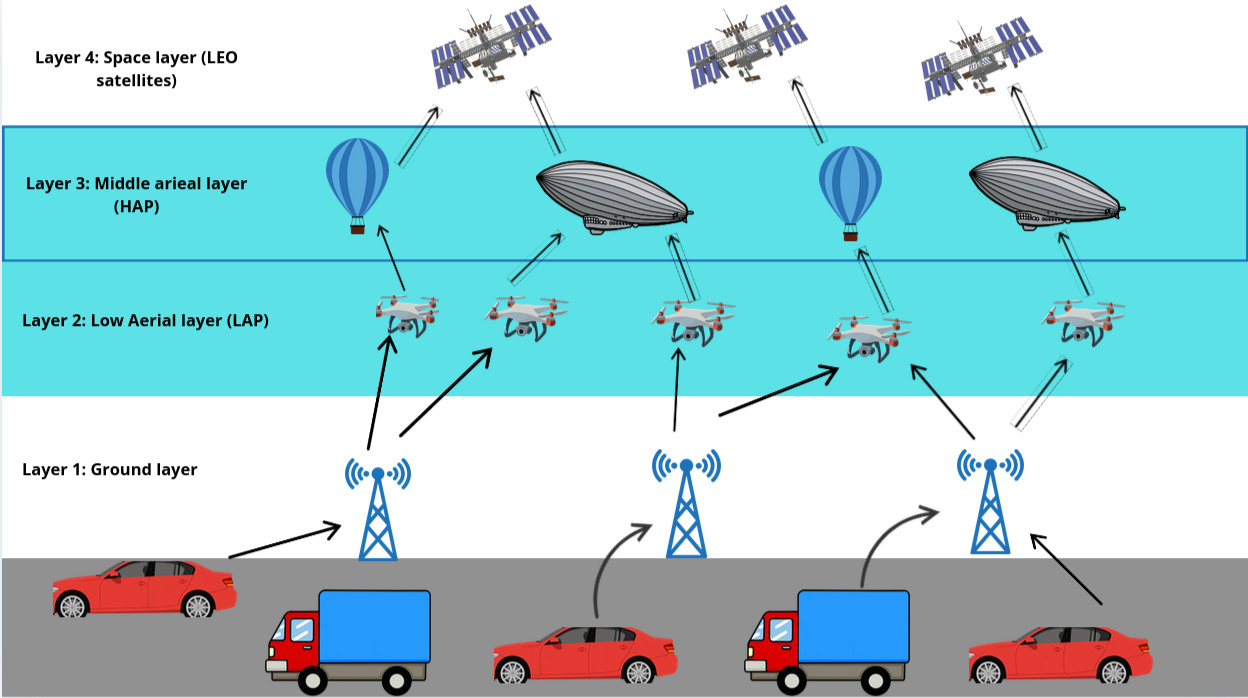
\includegraphics[width=\columnwidth]{network_scenario.jpg}
  \caption{The considered four-tier T-NTN scenario. Connected vehicles on the ground layer generate computational tasks and communicate via V2V/V2I links with Road-Side Units (Layer~1); offloading targets extend through the lower aerial layer of Low-Altitude Platforms (Layer~2, UAVs), the middle aerial layer of High-Altitude Platforms (Layer~3), up to the space layer of LEO satellites (Layer~4), with vehicle-to-aerial and inter-aerial links providing multi-hop connectivity across tiers.}
  \label{fig:scenario}
\end{figure}

We consider a T-NTN with four tiers indexed by $l \in \mathcal{L} = \{1,2,3,4\}$, as illustrated in Fig.~\ref{fig:scenario}: RSUs ($l=1$), LAPs ($l=2$), HAPs ($l=3$), and LEO satellites ($l=4$). Tier $l$ contains $M_l$ compute nodes, giving a total of $M = \sum_{l} M_l$ candidate offloading destinations. Additionally, one Cloud Computing facility $\mathcal{C}$ is located at ground level and accessible via backhaul from each edge node (EN); it can provide all services and is used as a fallback when the selected EN cannot serve the requested service type~\cite{hrl_ntn}.

At time slot $\tau_i$, vehicle $k$ generates task $x_k = (d_k, c_k, T_k^{\max}, \xi_k)$, where $d_k$ (bytes) is the payload size, $c_k$ (CPU cycles) the workload, $T_k^{\max}$ (s) the hard deadline, and $\xi_k \in \Xi$ the type of service requested. Each EN $e$ can serve only a subset $\Xi_e \subseteq \Xi$ of services. If the selected EN $e$ cannot serve $\xi_k$ (i.e.\ $\xi_k \notin \Xi_e$), it relays the task to $\mathcal{C}$, incurring additional communication and computation overhead; the binary indicator $b_e^{\xi_k} = \mathbf{1}[\xi_k \notin \Xi_e]$ flags this relay event.

\subsection{Communication Model}
\label{subsec:comm}

Following~\cite{hrl_ntn}, the channel gain between vehicle $k$ and any EN $e$ is modeled by distance-dependent path loss with a uniform formula across all tiers:
\begin{equation}
  h_{k,e}(i) = \eta_0 \cdot d_{k,e}(i)^{-\delta}
  \label{eq:channel_gain}
\end{equation}
where $d_{k,e}(i)$ is the Euclidean distance between vehicle $k$ and EN $e$ at slot $i$, $\eta_0$ the reference channel power gain at 1~m, and $\delta$ the path-loss exponent (whose value depends on the link type: ground-to-vehicle, air-to-ground, or satellite). The Shannon capacity of the $k$-to-$e$ link is
\begin{equation}
  R_{k,e}(i) = B_{k,e}(i)\,\log_2\!\left(1 + \frac{P_k\,h_{k,e}(i)}{N_0}\right)
  \label{eq:shannon}
\end{equation}
where $P_k$ is the vehicle transmit power, $B_{k,e}(i)$ the allocated bandwidth, and $N_0 = N_T B_{k,e}(i)$ the thermal noise power with spectral density $N_T$. A symmetric channel is assumed between any communicating pair~\cite{hrl_ntn}.

\subsection{Task Offloading Cost Model}
\label{subsec:cost}

For task $x_k$ with offloading fraction $\alpha_k \in [0,1]$ to EN $e$ in tier $l$, the \textbf{offloading latency} includes transmission, waiting, computation at $e$ (or cloud relay if $b_e^{\xi_k}=1$), and result reception:
\begin{equation}
  T_{k,\mathrm{off}}^{x_k}(i) = \alpha_k\!\left[T_{tx,ke}^{x_k} + T_{w,ke}^{x_k}
    + (1-b_e^{\xi_k})\,T_{c,ke}^{x_k} + T_{rx,ek}^{x_k}
    + b_e^{\xi_k}\!\left(T_{tx,e\mathcal{C}}^{x_k}
    + T_{w,\mathcal{C}}^{x_k} + T_{c,\mathcal{C}}^{x_k}
    + T_{rx,\mathcal{C}k}^{x_k}\right)\right]
  \label{eq:T_off}
\end{equation}
where $T_{tx}$, $T_w$, $T_c$, $T_{rx}$ denote transmission, waiting, computation, and receive times, respectively. The \textbf{local computation latency} for the non-offloaded fraction is
\begin{equation}
  T_{k,\mathrm{loc}}^{x_k}(i) = (1-\alpha_k)\,T_{c,kk}^{x_k}
  \label{eq:T_loc}
\end{equation}
with $T_{c,kk}^{x_k} = c_k / f_{v,k}$ the time to process the full task locally at CPU frequency $f_{v,k}$. Since partial offloading allows local and edge processing to run \emph{in parallel}, the \textbf{total task latency} is
\begin{equation}
  T^{x_k}\!\left(\alpha_k,\, a_{k,e}\right)
  = \max\!\left(T_{k,\mathrm{off}}^{x_k}(i),\; T_{k,\mathrm{loc}}^{x_k}(i)\right).
  \label{eq:latency}
\end{equation}
Define the VU and EN offloading energies as
\begin{align}
  E_{k,\mathrm{off}}^{x_k}(i) &= \alpha_k\!\left(E_{tx,ke}^{x_k} + E_{rx,ek}^{x_k}\right)
  \label{eq:E_koff}\\
  E_{e,\mathrm{off}}^{x_k}(i) &= \alpha_k\!\left[E_{w,ke}^{x_k}
    + (1-b_e^{\xi_k})\,E_{c,ke}^{x_k}
    + b_e^{\xi_k}\!\left(E_{tx,e\mathcal{C}}^{x_k}
    + E_{rx,\mathcal{C}e}^{x_k}\right)\right]
  \label{eq:E_eoff}
\end{align}
where $E_{tx}$, $E_{rx}$, $E_w$, $E_c$ are base energy costs for transmission, reception, waiting, and computation of the \emph{full} task. The \textbf{total energy cost} is~\cite{hrl_ntn}
\begin{equation}
  E^{x_k}\!\left(\alpha_k,\, a_{k,e}\right)
  = w_k\,E_{k,\mathrm{off}}^{x_k}(i)
  + E_{k,\mathrm{loc}}^{x_k}(i)
  + w_e\,E_{e,\mathrm{off}}^{x_k}(i)
  \label{eq:energy}
\end{equation}
where $w_k$ and $w_e$ are VU and EN energy-weighting coefficients, and the local computation energy is $E_{k,\mathrm{loc}}^{x_k}(i) = (1-\alpha_k)\,E_{c,kk}^{x_k}$, with $E_{c,kk}^{x_k}$ the energy to process the full task locally at the vehicle.

\subsection{Optimization Objective and Constraints}
\label{subsec:objective}

The system minimizes the weighted sum of latency and energy over all $K$ vehicles:
\begin{equation}
  \textbf{(P1):} \quad
  \min_{\{a_{k,e},\,\alpha_k\}}
  \;\frac{1}{K}\sum_{k=1}^{K}
  \Bigl[\beta_1\,T^{x_k}\!\left(\alpha_k,\,a_{k,e}\right)
       + \beta_2\,E^{x_k}\!\left(\alpha_k,\,a_{k,e}\right)\Bigr]
  \label{eq:P1}
\end{equation}
\begin{align}
  \text{s.t.} \quad
    & \sum_{e} a_{k,e} \leq 1, \quad \forall k
      \tag{C1}\label{eq:c1}\\
    & T^{x_k}\!\left(\alpha_k,\,a_{k,e}\right) \leq T_k^{\max}, \quad \forall k
      \tag{C2}\label{eq:c2}\\
    & T_{k,\mathrm{off}}^{x_k}(i) \leq T_{v_k,\mathrm{soj}}^{e}(i), \quad \forall k,e,i
      \tag{C3}\label{eq:c3}\\
    & E^{x_k}\!\left(\alpha_k,\,a_{k,e}\right) \leq w_k\,E_{c,kk}^{x_k}, \quad \forall k
      \tag{C4}\label{eq:c4}\\
    & 0 \leq \beta_1,\,\beta_2 \leq 1;\quad \beta_1 + \beta_2 = 1
      \tag{C5}\label{eq:c5}
\end{align}
where $a_{k,e} \in \{0,1\}$ is the binary EN-selection variable and $\beta_1, \beta_2$ are latency/energy weights. \textbf{C1} ensures each vehicle selects at most one EN. \textbf{C2} enforces the hard task deadline. \textbf{C3} requires offloading to complete before the vehicle leaves EN $e$'s coverage (sojourn constraint), with $T_{v_k,\mathrm{soj}}^{e}(i)$ the remaining sojourn time. \textbf{C4} bounds the total energy by that of full local processing, ensuring offloading is energetically justified. \textbf{C5} normalizes the weights. Problem (P1) is NP-hard owing to the mixed-integer structure and the non-convex coupling between the continuous $\alpha_k$ and the discrete $a_{k,e}$, which motivates the learning-based decomposition developed next.

\subsection{Evaluation Metrics}
\label{subsec:metrics}

The framework is assessed along five primary metrics---latency, energy consumption, reward, deadline-violation rate, and parameter count---each probing a distinct facet of the design; auxiliary learning and efficiency diagnostics are consolidated in Table~\ref{tab:metrics_summary}.

\begin{description}
  \item[Latency.] \emph{Definition:} the average per-task completion time $\bar T=\mathbb{E}[T^{x_k}]$ (s), with $T^{x_k}$ the end-to-end latency of Eq.~\eqref{eq:latency} (transmission, queueing, and compute, possibly via cloud relay). \emph{Why it matters:} latency is the primary service-quality target of~\eqref{eq:P1} and the quantity most directly perceived by latency-critical vehicular applications. \emph{What it evaluates:} the quality of the joint tier/ratio/node decision---the principal axis on which the quantum and classical policies are compared.
  \item[Energy consumption.] \emph{Definition:} the average per-task energy $\bar E=\mathbb{E}[E^{x_k}]$ (J) of Eq.~\eqref{eq:energy}, summing transmission, reception, and edge-compute energy for the offloaded fraction. \emph{Why it matters:} energy is the second objective in the cost~\eqref{eq:P1} and the dominant operational constraint for power-limited edge nodes. \emph{What it evaluates:} the cost side of the latency--energy trade-off, exposing whether a latency gain is bought with disproportionate energy.
  \item[Reward.] \emph{Definition:} the cumulative reward accrued by the agent over an evaluation episode, defined as the negative of the constrained offloading cost of~\eqref{eq:P1}---so that a higher reward corresponds to lower latency and energy and to fewer constraint violations. \emph{Why it matters:} reward is the scalar the learning agents actually optimise, so its trajectory captures convergence speed and stability in a single signal. \emph{What it evaluates:} the optimisation behaviour of each policy---how quickly and how stably it reaches a feasible, low-cost operating point. The exact discounted MDP return is formalised in Section~\ref{subsec:mdp}.
  \item[Deadline-violation rate.] \emph{Definition:} the fraction of tasks (in $\%$) whose end-to-end latency $T^{x_k}$ exceeds the hard deadline $T_k^{\max}$, i.e.\ that violate the deadline constraint~\eqref{eq:c2}. \emph{Why it matters:} a low mean latency is meaningful only if it is not obtained by sacrificing tail feasibility, so the deadline-miss rate is the feasibility counterpart of latency. \emph{What it evaluates:} the reliability of the policy under the hard real-time constraint, distinguishing genuinely feasible policies from those merely fast on average.
  \item[Parameter count.] \emph{Definition:} the number of trainable parameters $W$ of each method (VQC$+$QAOA angles for Quantum-HRL; network weights for the DQN baselines) and the reduction factor $\rho=W_{\mathrm{HRL}}/W_{\mathrm{Q\text{-}HRL}}$. \emph{Why it matters:} parameter count governs memory footprint, sample efficiency, and the conditioning of the optimisation, and is the headline efficiency claim of this work. \emph{What it evaluates:} the model compactness of the quantum policy relative to the classical pipeline---a footprint comparison, explicitly not a runtime speedup.
\end{description}

\noindent Beyond these five, Table~\ref{tab:metrics_summary} reports the remaining feasibility rates (the sojourn- and energy-budget-violation rates of constraints~\eqref{eq:c3} and~\eqref{eq:c4}), sample-efficiency and stability diagnostics (episodes-to-plateau $\Pi_\eta$ at $\eta{=}95$, seed-wise reward variance), and hardware-cost proxies (circuit evaluations per update, wall-clock per episode), each with its optimisation direction, so that every numerical entry in Section~\ref{sec:results} is unambiguous.

\begin{table}[t]
\centering
\small
\caption{Summary of evaluation metrics. $\downarrow$ indicates lower-is-better, $\uparrow$ higher-is-better.}
\label{tab:metrics_summary}
\begin{tabular}{@{}p{4.0cm}p{4.5cm}p{1.2cm}p{4.6cm}@{}}
\toprule
\textbf{Metric} & \textbf{Definition} & \textbf{Dir.} & \textbf{Purpose} \\
\midrule
Avg.\ task latency $\bar T$        & $\mathbb{E}[T^{x_k}]$ (s)                                & $\downarrow$ & Service quality \\
Avg.\ task energy $\bar E$         & $\mathbb{E}[E^{x_k}]$ (J)                                & $\downarrow$ & Energy efficiency \\
Deadline-miss rate                 & $\Pr(T^{x_k}{>}T_k^{\max})$ ($\%$)                       & $\downarrow$ & Feasibility under (C2) \\
Sojourn-violation rate             & Violation of~\eqref{eq:c3} ($\%$)                        & $\downarrow$ & Feasibility under (C3) \\
Energy-suboptimality rate          & Violation of~\eqref{eq:c4} ($\%$)                        & $\downarrow$ & Feasibility under (C4) \\
Cumulative reward                  & Discounted return ($-$cost of~\eqref{eq:P1})             & $\uparrow$   & Learning quality \\
Episodes-to-plateau $\Pi_\eta$     & Episodes to reach $\eta\%$ of asymptote ($\eta{=}95$)    & $\downarrow$ & Sample efficiency \\
Seed-wise reward variance          & $\mathrm{Var}_{\mathrm{seeds}}[\bar R]$                  & $\downarrow$ & Training stability \\
Trainable parameters $W$           & Total VQC$+$QAOA / DQN parameters                        & $\downarrow$ & Model compactness \\
Reduction factor $\rho$            & $W_{\mathrm{HRL}}/W_{\mathrm{Q\text{-}HRL}}$             & $\uparrow$   & Quantum compression \\
Circuit evaluations / update       & Counted per BO step (NISQ cost proxy)                    & $\downarrow$ & Hardware cost \\
Wall-clock / episode               & Seconds on the simulated back-end                        & $\downarrow$ & Practicality \\
\bottomrule
\end{tabular}
\end{table}

%=============================================================================
% V. PROPOSED FRAMEWORK
%=============================================================================
\section{Proposed Framework}
\label{sec:framework}

We first describe the classical HRL baseline that defines the problem decomposition (Section~\ref{subsec:classical}), then the proposed Quantum-HRL framework that replaces it (Section~\ref{subsec:qhrl}), the MDP formulation underlying both (Section~\ref{subsec:mdp}), the QUBO mapping that enables QAOA-based node selection (Section~\ref{subsec:qubo}), and finally the training strategy (Section~\ref{subsec:training}).

\subsection{Classical HRL Baseline}
\label{subsec:classical}

The classical baseline of Shinde and Tarchi~\cite{hrl_ntn} solves (P1) by decomposing the joint decision into three sub-problems handled by three sequential Deep $Q$-Networks (DQNs), each trained on the temporal-difference error of its $Q$-values:
\begin{itemize}
  \item \textbf{Layer (tier) selection.} A master DQN maps the state $s_t\in\R^n$ to $Q$-values over the $|\mathcal L|=4$ tiers and selects $l_t=\argmax_l Q^{(1)}(s_t,l)$. This sets the macroscopic offloading target (RSU/LAP/HAP/LEO).
  \item \textbf{Node selection.} Conditioned on the chosen tier, a worker DQN treats the $M_{l_t}$ candidate nodes as a flat discrete action set and selects $n_t=\argmax_n Q^{(2)}(s_t,n)$. The combinatorial assignment is thus represented as a tabular $Q$-value lookup.
  \item \textbf{Ratio selection.} A second worker DQN selects the offloading ratio $\alpha_t$ from $K_\alpha$ discretized levels, $\alpha_t=\argmax_\alpha Q^{(3)}(s_t,\alpha)$, determining how much of the workload is offloaded versus processed locally.
\end{itemize}
The three networks are coordinated sequentially---the node and ratio heads consume the tier decision---and each is duplicated into a primary and a target copy for stable DQN training. This decomposition is effective and constitutes a strong, learned baseline, but it inherits the three structural limitations identified in Section~\ref{sec:intro}: an $O(n\cdot h)$ parameter cost per head, a node selector that ignores the algebraic structure of the assignment problem, and sequential-coordination friction. The detailed parameter accounting is given in Section~\ref{subsec:complexity}.

\subsection{Proposed Quantum-HRL Framework}
\label{subsec:qhrl}

\paragraph{From classical HRL to Quantum-HRL.}
The tri-DQN baseline is effective but exposes three structural limitations that motivate a quantum redesign rather than incremental tuning, and each limitation maps to one component of the proposed framework. \emph{(i)~Parameter cost.} Every head is a fully-connected network whose input layer alone costs $O(n\cdot h)$ weights, duplicated into primary and target copies and replicated across three heads, so the model grows linearly with the state dimension---wasteful for the compact, structured states of T-NTN offloading. We therefore replace the two high-level heads with a single \emph{variational quantum circuit}: amplitude encoding loads the $n$-dimensional state into $\lceil\log_2 n\rceil$ qubits, so a depth-$L$ VQC parameterises the tier/ratio policy with only $O(L\log_2 n)$ angles---an exponential reduction in the input-coupling cost while retaining a differentiable, gradient-trainable policy. \emph{(ii)~Unstructured node selection.} The node head treats the $M_l$ candidate nodes as a flat categorical action and learns one tabular $Q$-value per node, ignoring that node selection is a \emph{constrained combinatorial assignment}---exactly one node must be chosen, and the per-node cost is a known function of the channel and load state. Casting it as a one-hot quadratic program (Section~\ref{subsec:qubo}) makes this algebraic structure explicit and recoverable by a dedicated solver. \emph{(iii)~Re-learning under drift.} Because the per-node costs are rebuilt every slot from the current state, a learned $Q$-table must continually re-adapt as costs drift; a \emph{stateless} optimiser that consumes the cost directly is preferable. This is precisely what \emph{QAOA} provides: it solves the QUBO/Ising form of the assignment with a constant $2p$ angles independent of $M_l$, enforcing the one-hot constraint through the cost Hamiltonian itself. The net effect is an architecture that scales \emph{logarithmically} in the state dimension (via the VQC) and \emph{constantly} in the node count (via QAOA), in contrast to the linear growth of the tri-DQN, while preserving the hierarchical tier\,$\to$\,node\,$\to$\,ratio decomposition that makes the baseline effective.

Quantum-HRL replaces the three-DQN pipeline with a hybrid quantum-classical system composed of four integrated modules---quantum state encoding, a VQC-based high-level policy, a QAOA-based low-level combinatorial optimiser, and a Bayesian-Optimisation outer loop---as illustrated in Fig.~\ref{fig:architecture}. Classical and quantum subroutines are coupled through a single MDP loop so that policy updates remain consistent with the offloading cost and reward signals of Section~\ref{sec:problem}.

\begin{figure}[htbp]
  \centering
  
\includegraphics[width=0.8\columnwidth]{system_architecture.png}
  \caption{Architecture comparison between the classical HRL baseline and the proposed Quantum-HRL framework. The classical pipeline (left) routes the state $s_t$ through three sequential DQNs for layer, ratio, and node selection, totalling $20{,}224$ trainable parameters. Quantum-HRL (right) replaces them with an amplitude-encoded VQC high-level policy (tier and ratio) followed by a QAOA node selector acting on the node-selection QUBO, reducing the trainable-parameter count to $24$ while preserving the hierarchical decomposition.}
  \label{fig:architecture}
\end{figure}

\paragraph{Amplitude encoding (state loading).}
At each slot $\tau_i$, the environment snapshot $s_t \in \R^n$ is mapped to a quantum state via Amplitude Encoding~\cite{biamonte2017qml}. Given the normalized vector $\tilde{s}_t = s_t / \norm{s_t}$ (Corollary~\ref{cor:norm}), we prepare
\begin{equation}
  \ket{\psi(s_t)} = \sum_{i=0}^{n-1} \tilde{s}_t^{(i)} \ket{i},
  \label{eq:amplitude_encoding}
\end{equation}
which requires only $\lceil \log_2 n \rceil$ qubits to represent the $n$-dimensional state---the compact input representation that underlies the framework's parameter efficiency.

\paragraph{VQC high-level policy (layer and ratio selection).}
The encoded state $\ket{\psi(s_t)}$ is processed by the VQC $U(\theta)$ of Eq.~\eqref{eq:vqc_def}, which functions as the high-level policy $\pi_\theta$ and jointly produces two outputs from measurements of Pauli-$Z$ observables:
\begin{itemize}
  \item \textbf{Layer selection:} $l^* = \argmax_{l \in \mathcal{L}} \langle \hat{O}_l \rangle$, the tier maximizing the expectation of a layer-specific observable $\hat{O}_l$.
  \item \textbf{Offloading ratio:} $\alpha = \sigma(\langle \hat{O}_\alpha \rangle)$, with $\sigma(\cdot)$ the logistic function applied to a dedicated readout observable $\hat{O}_\alpha$.
\end{itemize}
A single VQC therefore subsumes both the tier and ratio heads of the classical baseline. The qc-level circuit structure (rotation--entanglement layers, amplitude-encoded input, and dual readout) is depicted in Fig.~\ref{fig:vqc}.

\begin{figure}[t]
  \centering
  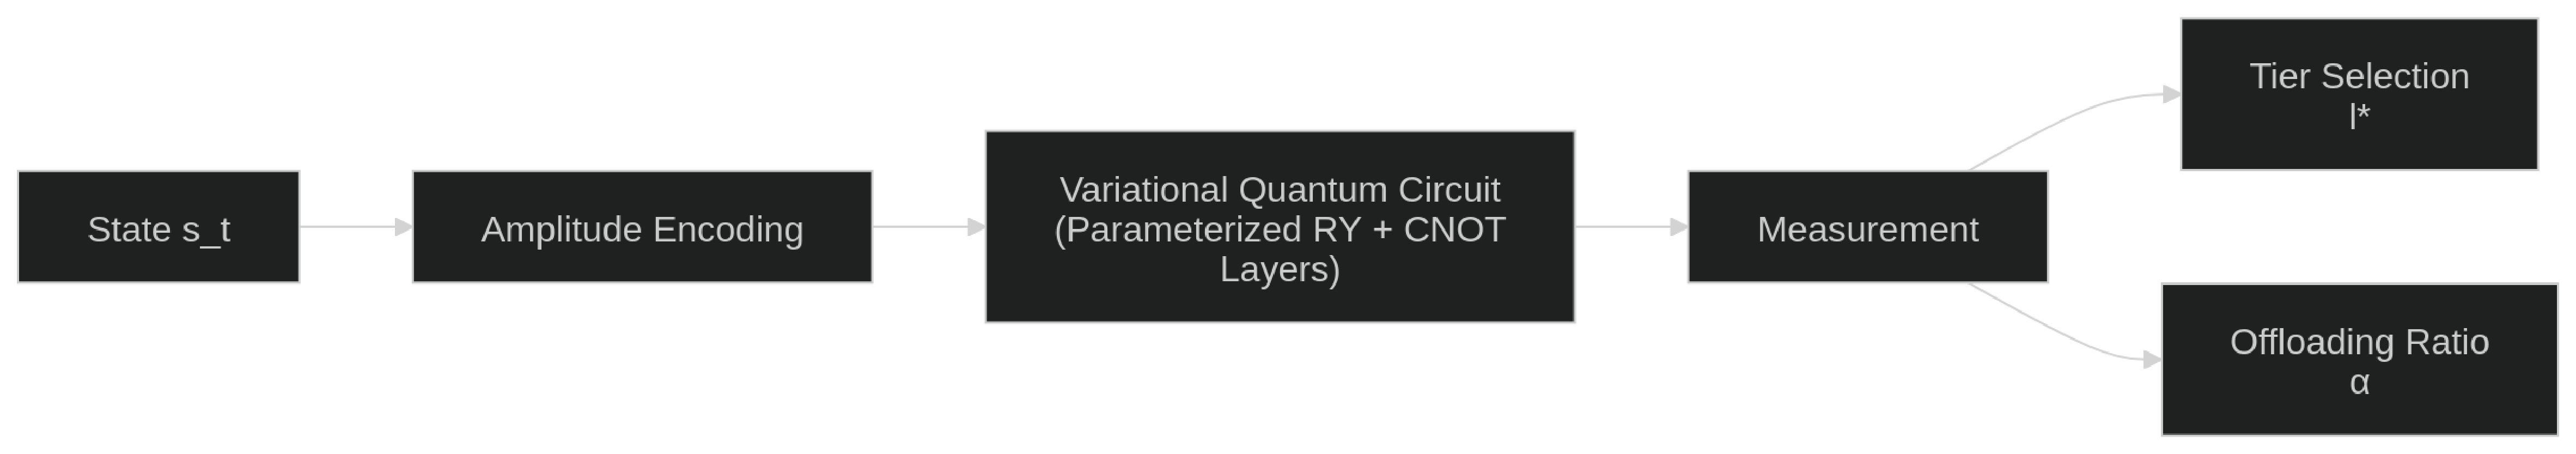
\includegraphics[width=0.92\columnwidth]{qc1_vqc_architecture.pdf}
  \caption{VQC architecture used as the high-level policy. The amplitude-encoded state on $q=\lceil\log_2 n\rceil$ qubits is processed by $L$ alternating layers of parameterized $R_Y$ rotations and CNOT entanglers; Pauli-$Z$ expectation values feed a softmax tier readout (layer selection $l^*$) and a sigmoid ratio readout ($\alpha$).}
  \label{fig:vqc}
\end{figure}

\paragraph{QAOA low-level optimiser (node selection).}
Once $(l^*,\alpha)$ is fixed, node selection within tier $l^*$ is solved by QAOA on the cost Hamiltonian built from the node-selection QUBO (Section~\ref{subsec:qubo}). Running the depth-$p$ circuit of Eq.~\eqref{eq:qaoa_def} and measuring in the computational basis yields the bitstring $z^*$ that identifies $n^* = \argmax_n z_n^*$.

\begin{remark}[Hierarchical ordering rationale]
The classical baseline~\cite{hrl_ntn} sequences decisions as tier $\to$ node $\to$ ratio, so the ratio is optimized after the node is known. Quantum-HRL instead collapses tier and ratio into a single VQC step, then resolves node selection via QAOA. This ordering is self-consistent: the QAOA cost Hamiltonian uses $c_n(\alpha)=\beta_1 T_{k,n}(\alpha)+\beta_2 E_{k,n}(\alpha)$, so node selection is performed \emph{conditioned on} the ratio $\alpha$ already output by the VQC. The VQC therefore learns a policy globally consistent with downstream node costs, while QAOA optimizes the combinatorial assignment given the fixed context $(l^*,\alpha)$.
\end{remark}

\paragraph{End-to-end loop.}
The composite action $a_t=(l^*,n^*,\alpha)$ is executed in the environment, which returns latency $T^{x_k}$, energy $E^{x_k}$, and the constraint flags used to compute the reward. The reward then drives the VQC policy-gradient update and the Bayesian-Optimisation refinement of the QAOA angles (Section~\ref{subsec:training}). The complete decision-and-learning cycle is shown in Fig.~\ref{fig:decision_flow} and summarised in Algorithm~\ref{alg:quantum_hrl}.

\begin{figure}[htbp]
  \centering
  
\includegraphics[width=0.58\columnwidth]{quantum_hrl_decision_flow.png}
  \caption{End-to-end Quantum-HRL decision pipeline. The task-offloading problem---latency, energy, and resource constraints---is cast as an MDP (state, action, reward); its node-selection sub-problem is then expressed with binary variables, mapped to a QUBO and its Ising Hamiltonian, and solved by QAOA to return the optimal node. The high-level VQC policy and the QAOA node selector jointly yield the final composite decision $(l^*,n^*,\alpha)$.}
  \label{fig:decision_flow}
\end{figure}

\begin{algorithm}[t]
\caption{Quantum-HRL for T-NTN Task Offloading}
\label{alg:quantum_hrl}
\begin{algorithmic}[1]
\Require T-NTN environment; VQC depth $L$; QAOA depth $p$; BO budget $B$
\Ensure Optimized parameters $\theta^*$, $(\gamma^*, \beta^*)$
\State Initialize $\theta$, $\gamma$, $\beta$ randomly; replay buffer $\mathcal{D} \leftarrow \emptyset$
\For{each episode}
  \State Observe state $s_t$; normalize to $\tilde{s}_t$
  \State Encode: $\ket{\psi(s_t)} \leftarrow$ Amplitude Encoding($\tilde{s}_t$)
  \State \textbf{High-level}: Measure $U(\theta)\ket{\psi(s_t)}$ $\to$ $(l^*, \alpha)$ \Comment{VQC}
  \State Construct cost Hamiltonian $H_C$ for layer $l^*$
  \State \textbf{Low-level}: Run QAOA$(\gamma, \beta)$ on $H_C$ $\to$ $n^*$ \Comment{QAOA}
  \State Execute action $a_t = (l^*, n^*, \alpha)$; observe $R_t$, $s_{t+1}$
  \State Store $(s_t, a_t, R_t, s_{t+1})$ in $\mathcal{D}$
  \If{$|\mathcal{D}|$ mod $B$ = 0}
    \State Update $\theta$ via advantage-weighted PSR policy gradient on a batch from $\mathcal{D}$ \Comment{Eq.~\eqref{eq:vqc_pg}}
    \State Update $(\gamma, \beta)$ via BO on QAOA cost landscape
  \EndIf
\EndFor
\end{algorithmic}
\end{algorithm}

\subsection{MDP Formulation}
\label{subsec:mdp}

Sequential task offloading is naturally modeled as a Markov Decision Process (MDP): the controller observes the current network state, takes an action, receives a reward reflecting latency, energy, and feasibility, and transitions to a new state as vehicles move and loads evolve---a memoryless, slot-by-slot decision process for which RL provides adaptive policies without an explicit environment model. We cast (P1) as an MDP $(\mathcal{S}, \mathcal{A}, \mathcal{R}, \gamma_{\mathrm{MDP}})$ following the hierarchical decomposition of~\cite{hrl_ntn}:
\begin{itemize}
  \item \textbf{State} $s_t \in \mathbb{R}^n$: a concatenation of (i)~vehicle position and velocity, (ii)~per-node CPU load $\{u_{l,n}^t\}$, (iii)~channel gains $\{h_{k,e}^t\}$, (iv)~layer-wise average VU count and EN mobility estimate, and (v)~task parameters $(d_k, c_k, T_k^{\max}, \xi_k)$. The state dimension is $n = 20$ for the configuration of Section~\ref{sec:experimental}.
  \item \textbf{Action} $a_t = (l_t, n_t, \alpha_t)$: jointly selected tier $l_t \in \mathcal{L}$, edge node $n_t \in \{1,\ldots,M_{l_t}\}$, and offloading ratio $\alpha_t \in [0,1]$.
  \item \textbf{Reward} $R_t$: minimizes latency and energy while penalizing violations of three operational constraints inherited from~\cite{hrl_ntn}.
\end{itemize}

Define three binary constraint-violation indicators following~\cite{hrl_ntn}:
\begin{align}
  F^1_{k,e}(t) &= \mathbf{1}\!\left[T_{k,\mathrm{off}}^{x_k}(i) > T_{v_k,\mathrm{soj}}^{e}(i)\right]
  \label{eq:f1} \\
  F^2_{k,e}(t) &= \mathbf{1}\!\left[T^{x_k}\!\left(\alpha_k,\,a_{k,e}\right) > T_k^{\max}\right]
  \label{eq:f2} \\
  F^3_{k,e}(t) &= \mathbf{1}\!\left[E^{x_k}\!\left(\alpha_k,\,a_{k,e}\right) > w_k\,E_{c,kk}^{x_k}\right]
  \label{eq:f3}
\end{align}
where $T_{v_k,\mathrm{soj}}^{e}(i)$ is the sojourn-time bound, $T_k^{\max}$ the hard deadline, and $w_k E_{c,kk}^{x_k}$ the energy of fully local processing---so $F^3=1$ signals that offloading is \emph{less} energy-efficient than local computation, violating~\eqref{eq:c4}. The reward is the negated cost of~\eqref{eq:P1} augmented with constraint penalties:
\begin{equation}
  R_t = -\!\left(\beta_1\,T^{x_k} + \beta_2\,E^{x_k}\right)
        - w_1 F^1_{k,e}(t)
        - w_2 F^2_{k,e}(t)
        - w_3 F^3_{k,e}(t),
  \label{eq:reward}
\end{equation}
where $w_1, w_2, w_3 > 0$ are penalty magnitudes for sojourn, deadline, and energy violations, and the negation converts the minimization objective into the standard RL maximization of $\mathbb{E}[\sum_t \gamma_{\mathrm{MDP}}^t R_t]$. Setting $w_i \gg \max(\beta_1 T^{x_k} + \beta_2 E^{x_k})$ ensures feasibility is prioritized over cost.

\subsection{QUBO Mapping for Node Selection}
\label{subsec:qubo}

The node-selection sub-problem is the key combinatorial component delegated to QAOA. We derive its mapping in four steps: optimization problem $\to$ binary formulation $\to$ QUBO $\to$ Ising Hamiltonian, after which QAOA (Section~\ref{subsec:bg_qaoa}) consumes the Hamiltonian directly.

\paragraph{Why a QUBO formulation.}
Before deriving the mapping we motivate why node selection is recast as a QUBO rather than optimised directly. \emph{Direct optimisation is awkward.} Node selection is an integer program---choose exactly one of $M_{l^*}$ discrete nodes to minimise a cost $c_n(\alpha)$ that is rebuilt every slot from the channel and load state. The feasible set is discrete and non-convex, gradient methods do not apply to the selection variable, and exhaustive enumeration, while tractable for small tiers, scales poorly as node populations grow and must be repeated from scratch at every slot; a representation that exposes the combinatorial structure to a structure-aware solver is therefore preferable. \emph{Binary variables make the structure explicit.} Encoding the decision as indicators $z_n\in\{0,1\}$ with $z_n{=}1$ iff node $n$ is selected turns ``choose one node'' into the linear one-hot constraint $\sum_n z_n=1$ and the objective into a function of the $z_n$, so the combinatorial choice becomes an algebraic object that can be penalised and manipulated. \emph{QUBO is the right algebraic form.} A quadratic unconstrained binary optimisation absorbs the one-hot constraint as a quadratic penalty, yielding a single unconstrained quadratic in $z$ with no separate feasibility handling---constraint satisfaction is folded into the objective. QUBO is moreover the canonical input format for a broad class of combinatorial solvers, so the same formulation is portable across classical heuristics and quantum optimisers. \emph{QAOA requires a QUBO.} QAOA operates on a cost Hamiltonian obtained from the change of variable $z_n=(I-\hat\sigma_n^z)/2$, which maps a QUBO exactly onto an Ising model; the algorithm has no other interface to the problem. A QUBO formulation is thus not merely convenient but \emph{necessary} to bring node selection into the QAOA framework, and the one-hot penalty becomes the quadratic spin coupling that enforces feasibility on the device. The four-step derivation below makes this chain precise.

\paragraph{Step 1: optimization problem.}
Given a fixed tier $l^*$ and ratio $\alpha$, node selection reduces to
\[
  n^* = \argmin_n \big[\beta_1\,T^{x_k}(\alpha, a_{k,n}) + \beta_2\,E^{x_k}(\alpha, a_{k,n})\big],
\]
with $T^{x_k}$ and $E^{x_k}$ evaluated via Eqs.~\eqref{eq:latency} and~\eqref{eq:energy} at the VQC-fixed ratio $\alpha$.

\paragraph{Step 2: binary formulation.}
Introduce binary variables $z \in \{0,1\}^{M_{l^*}}$ with $z_n = 1$ iff node $n$ is chosen, subject to the one-hot constraint $\sum_n z_n = 1$.

\paragraph{Step 3: QUBO.}
A Quadratic Unconstrained Binary Optimization (QUBO) problem has the general form $\min_{z\in\{0,1\}^m} z^\top Q z + c^\top z$, where constraints enter as quadratic penalties. Encoding the per-node cost and the one-hot constraint yields
\begin{equation}
  \min_{z} \;\mathcal{H}(z) = \sum_{n=1}^{M_{l^*}} c_n z_n + A\!\left(\sum_{n=1}^{M_{l^*}} z_n - 1\right)^{\!2},
  \label{eq:qubo}
\end{equation}
where $c_n \triangleq \beta_1 T^{x_k}(\alpha, a_{k,n}) + \beta_2 E^{x_k}(\alpha, a_{k,n})$ is the per-node cost and the penalty $A \gg \max_n c_n$ enforces the one-hot constraint.

\paragraph{Step 4: Ising Hamiltonian.}
Substituting $z_n = \tfrac{I - \hat{\sigma}_n^z}{2}$ (Pauli-$Z$ mapping, with $\hat{\sigma}_n^z\ket{0}=+\ket{0}$, $\hat{\sigma}_n^z\ket{1}=-\ket{1}$) and expanding gives the Ising-form cost Hamiltonian consumed by QAOA:
\begin{equation}
  H_C = \sum_{n=1}^{M_{l^*}} h_n\,\hat{\sigma}_n^z
        + \frac{A}{2}\!\sum_{n < m}\!\hat{\sigma}_n^z\hat{\sigma}_m^z + E_0,
  \label{eq:hamiltonian}
\end{equation}
with local fields, couplings, and constant offset
\begin{equation}
  h_n = -\frac{c_n}{2} + A\!\left(1 - \frac{M_{l^*}}{2}\right),
  \quad
  J_{nm} = \frac{A}{2},
  \quad
  E_0 = \sum_n \frac{c_n}{2} + A\!\left(1 - \frac{M_{l^*}}{2} + \frac{M_{l^*}(M_{l^*}-1)}{4}\right).
  \label{eq:ising_coeffs}
\end{equation}
The positive coupling $J_{nm} = +A/2 > 0$ penalises states where two or more spins simultaneously reach $-1$ (two nodes co-selected), enforcing the one-hot constraint. The ground state of $H_C$ identifies the minimum-cost node. Figure~\ref{fig:ising} illustrates the full chain from the optimization objective through the MDP to the QUBO and its Ising/QAOA realization.

\begin{figure}[t]
  \centering
  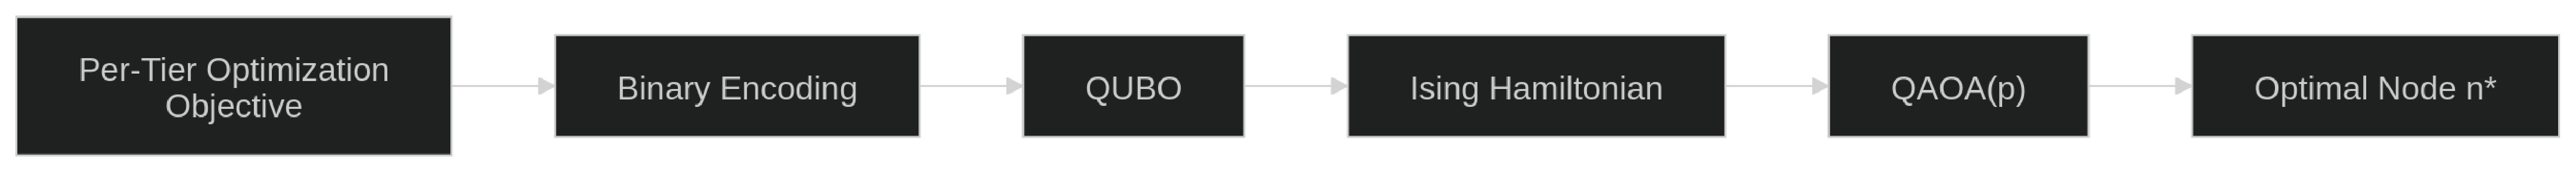
\includegraphics[width=0.95\columnwidth]{qc4_ising_mapping.pdf}
  \caption{Mapping of the node-selection problem: the per-tier optimization objective is recast as a binary one-hot QUBO~\eqref{eq:qubo}, mapped to an Ising cost Hamiltonian~\eqref{eq:hamiltonian} via the Pauli-$Z$ substitution, and solved by the depth-$p$ QAOA circuit whose ground state encodes the selected node $n^*$.}
  \label{fig:ising}
\end{figure}

\paragraph{Why QAOA is suitable.}
The node-selection instance has three properties that make QAOA a natural fit. First, it is a genuine combinatorial problem with a one-hot feasibility constraint that maps exactly onto the quadratic Ising couplings in~\eqref{eq:ising_coeffs}, so the constraint is enforced by the Hamiltonian rather than by post-processing. Second, the instance is rebuilt from scratch at every slot from the current per-node costs $c_n(\alpha)$, so a \emph{stateless} solver that consumes the Hamiltonian directly is preferable to a tabular $Q$-function that must be re-learned as costs drift. Third, by Proposition~\ref{prop:qaoa_convergence} the QAOA parameter count is $2p$ regardless of $M_{l^*}$, so the low-level optimiser does not inflate the model footprint as the node population grows---in contrast to the flat $Q$-table of the classical baseline.

\subsection{Training Strategy}
\label{subsec:training}

Quantum-HRL separates training into a classical component (the baseline DQNs, for reference) and a quantum component (the VQC and QAOA modules), each updated by the rule appropriate to its parameter landscape. We describe the quantum training in five steps; the global reward $R_1$ trains the VQC and the intrinsic node reward $R_2$ scores QAOA.

\paragraph{Classical training (baseline).}
For completeness, the classical baseline of Section~\ref{subsec:classical} trains each of its three DQNs by stochastic gradient descent on the temporal-difference error of the $Q$-values, with experience replay and a periodically-synchronised target network per head~\cite{hrl_ntn,mnih2015dqn}. This is the standard value-based update and is included only as the comparison point for the quantum training below.

\paragraph{Step 1: action selection.}
At each step $t$, the VQC defines a \emph{stochastic} high-level policy: the tier is sampled from $\pi_\theta(l \mid s_t) = \mathrm{softmax}(\langle\hat O_1\rangle,\ldots,\langle\hat O_{|\mathcal L|}\rangle)_l$ and the ratio from a Gaussian policy $\alpha \sim \mathcal N(\mu_\theta(s_t), \sigma_\alpha^2)$ clipped to $(0,1]$, where $\mu_\theta(s_t) = \sigma(\langle\hat O_\alpha\rangle)$. Training-time exploration is provided directly by this on-policy sampling; at evaluation the policy acts greedily ($l^* = \argmax_l \pi_\theta$, $\alpha = \mu_\theta$). QAOA is then invoked to select node $n^*$ within tier $l^*$.

\paragraph{Step 2: reward computation.}
After executing $(l^*, n^*, \alpha)$, the environment returns $T^{x_k}$ and $E^{x_k}$, and the three constraint flags of Eqs.~\eqref{eq:f1}--\eqref{eq:f3} are evaluated. Two reward signals are computed:
\begin{align}
  R_1^t &= -\!\left(\beta_1\,T^{x_k} + \beta_2\,E^{x_k}\right)
           - w_1 F^1 - w_2 F^2 - w_3 F^3
           \label{eq:r1} \\[4pt]
  R_2^t &= -\!\left(\beta_1\,T^{x_k}(\alpha, a_{k,n^*})
           + \beta_2\,E^{x_k}(\alpha, a_{k,n^*})\right)
           - w_2 F^2 - w_3 F^3
           \label{eq:r2}
\end{align}
$R_1^t$ (\textbf{global reward}) penalizes the full joint cost and all three violations and trains the VQC. $R_2^t$ (\textbf{intrinsic node reward}) isolates node selection (holding tier and ratio fixed), omits the sojourn penalty $w_1 F^1$ (a mobility side effect, not attributable to node quality), and scores QAOA. Table~\ref{tab:reward_routing} summarizes the routing.

\begin{table}[htbp]
\centering
\caption{Reward--component coupling in Quantum-HRL.}
\label{tab:reward_routing}
\begin{tabular}{@{}llll@{}}
\toprule
\textbf{Signal} & \textbf{Formula} & \textbf{Penalty terms} & \textbf{Trains} \\
\midrule
$R_1$ (global) & $-(\beta_1 T^{x_k} {+} \beta_2 E^{x_k}) {-} \sum_i w_i F^i$ & $F^1, F^2, F^3$ & VQC ($\theta$) \\
$R_2$ (intrinsic) & $-(\beta_1 T^{x_k}(\alpha,n^*) {+} \beta_2 E^{x_k}(\alpha,n^*)) {-} w_2 F^2 {-} w_3 F^3$ & $F^2, F^3$ & QAOA ($\gamma, \beta$) \\
\bottomrule
\end{tabular}
\end{table}

\noindent\textbf{Penalty magnitude rule.} To ensure feasibility is always prioritized over cost, penalty weights satisfy
\begin{equation}
  w_i \;\gg\; \max_{k,t}\!\left(\beta_1 T_k + \beta_2 E_k\right),
  \quad i \in \{1,2,3\}.
  \label{eq:penalty_rule}
\end{equation}
In practice each $w_i$ is set to the empirical 99th percentile of $(\beta_1 T_k + \beta_2 E_k)$ measured during a random-policy warm-up, so even a single violation dominates the reward signal.

\paragraph{Step 3: transition storage.}
The tuple $(s_t, l^*, n^*, \alpha, R_1^t, R_2^t, s_{t+1})$ is appended to the replay buffer $\mathcal{D}$. As in the baseline DQN memories~\cite{hrl_ntn}, the buffer breaks temporal correlations between consecutive samples and enables stable off-policy learning.

\paragraph{Step 4: VQC update via REINFORCE with the parameter-shift rule (every $B$ steps).}
A mini-batch of $k$ transitions is sampled and the VQC policy is updated by \textbf{advantage-weighted policy gradient} (REINFORCE with a batch-mean baseline), following the quantum policy-gradient formulation of~\cite{jerbi2021policies,sequeira2023policygradient}. The normalised advantage is
\begin{equation}
  \hat A_t \;=\; \frac{R_1^t - \bar R_1}{\mathrm{std}(R_1) + \epsilon},
  \qquad \bar R_1 = \tfrac1k\textstyle\sum_{\mathcal D} R_1^t,
  \label{eq:advantage}
\end{equation}
and the ascent direction is the advantage-weighted gradient of the log-policy,
\begin{equation}
  \nabla_\theta J(\theta)
  \;=\; \frac1k \sum_{\mathcal D} \hat A_t
  \Bigl[\, \nabla_\theta \log \pi_\theta(l^*_t \mid s_t)
        \;+\; \nabla_\theta \log \mathcal N\!\bigl(\alpha_t;\, \mu_\theta(s_t), \sigma_\alpha^2\bigr) \Bigr].
  \label{eq:vqc_pg}
\end{equation}
Both log-policy gradients reduce, via the chain rule through the softmax and sigmoid readouts, to linear combinations of the observable gradients $\partial\langle\hat O_k\rangle/\partial\theta_j$, each computed \emph{exactly} by the Parameter-Shift Rule (Eq.~\eqref{eq:psr})---no backpropagation through quantum operations is required. Normalising the advantage is essential on quantum hardware: the raw return $R_1$ (with penalty terms of magnitude $w_i$) is unbounded, whereas all circuit outputs are Pauli-$Z$ expectations confined to $[-1,1]$; the normalised advantage makes the update scale-free and keeps the bounded readouts well-conditioned.

\paragraph{Step 5: QAOA update via Bayesian Optimization (every $B$ steps).}
The QAOA angles $(\gamma, \beta)$ are \emph{not} updated by the policy gradient. Instead they are optimized by Bayesian Optimization (Section~\ref{subsec:bg_bo}) to minimize the expected QAOA energy for the cost Hamiltonian built from $R_2$ feedback:
\begin{enumerate}
  \item Compute the \textbf{empirical node cost} $\hat{c}_n = -\mathbb{E}_\mathcal{D}[R_2^t \mid n^* = n]$ from recent $R_2$ samples (average intrinsic reward received when node $n$ was selected).
  \item Rebuild the \textbf{cost Hamiltonian} $H_C$ using $\hat{c}_n$ as node costs in Eq.~\eqref{eq:qubo}.
  \item Run \textbf{Bayesian Optimization} to minimize $C(\gamma, \beta) = \bra{\gamma,\beta} H_C \ket{\gamma,\beta}$, updating the GP surrogate and proposing the next $(\gamma, \beta)$ via Expected Improvement~\eqref{eq:ei_def}.
\end{enumerate}
QAOA therefore learns \emph{which nodes are genuinely good} from accumulated experience (via $R_2$) rather than from the instantaneous cost Hamiltonian alone; minimizing $C(\gamma,\beta)$ drives the measured bitstring distribution toward $n^* = \argmin_n \hat{c}_n$. Table~\ref{tab:penalty_effect} summarizes the training-dynamics effect of each penalty.

\begin{table}[htbp]
\centering
\caption{Penalty terms and their training effect.}
\label{tab:penalty_effect}
\begin{tabular}{@{}p{1.6cm}p{2.8cm}p{3.5cm}p{4.2cm}@{}}
\toprule
\textbf{Penalty} & \textbf{Activates when} & \textbf{Effect on $R_1$} & \textbf{Policy correction induced} \\
\midrule
$w_1 F^1$ & Vehicle leaves coverage before offload completes ($T_k > T_k^{\mathrm{soj}}$) &
$R_1$ drops by $w_1$ &
VQC learns to prefer lower tiers (RSU/LAP) with shorter sojourn delays, or reduce $\alpha$ \\[6pt]
$w_2 F^2$ & Task misses hard deadline ($T_k > T_k^{\max}$) &
$R_1$ and $R_2$ both drop by $w_2$ &
VQC lowers $\alpha$ or selects a faster tier; QAOA favors nodes with lower $T_{k,n}$ \\[6pt]
$w_3 F^3$ & Offloading less energy-efficient than local ($E^{x_k} > w_k E_{c,kk}^{x_k}$) &
$R_1$ and $R_2$ both drop by $w_3$ &
VQC reduces $\alpha$ (less transmission energy); QAOA avoids distant nodes with high path loss \\
\bottomrule
\end{tabular}
\end{table}

%=============================================================================
% VI. EXPERIMENTAL DESIGN
%=============================================================================
\section{Experimental Design}
\label{sec:experimental}

This section specifies the construction of the evaluation dataset (Section~\ref{subsec:setup}), the hardware and software configuration (Section~\ref{subsec:config}), and the experimental scenarios (Section~\ref{subsec:scenarios}). The same data-input, processing, decision, and output pipeline is applied to every method under comparison; only the high-level/low-level policy is swapped, isolating the contribution of the proposed framework.

\subsection{Dataset Construction}
\label{subsec:setup}

The evaluation dataset is constructed by composing three independently sourced components into a single, internally consistent T-NTN offloading benchmark: (i)~a \emph{realistic vehicular-mobility layer} drawn from the Luxembourg SUMO Traffic (LuST) scenario~\cite{codeca2015lust}; (ii)~a \emph{task-workload layer} adopted from the classical HRL baseline of Shinde and Tarchi~\cite{hrl_ntn}; and (iii)~a \emph{network-parameter layer}---topology, channel, and per-tier characteristics---likewise adopted from~\cite{hrl_ntn}. The three layers are orthogonal and combine at the granularity of a decision slot $\tau_i$: the mobility layer fixes \emph{where} each vehicle is and \emph{how} it moves, the workload layer fixes \emph{what} each vehicle requests, and the network layer fixes the \emph{propagation and compute conditions} under which the request must be served. Their composition yields the per-slot state $s_t$ of Section~\ref{subsec:mdp} and the latency/energy cost of Section~\ref{sec:problem}.

\paragraph{Mobility layer (LuST).}
Realistic mobility is obtained from the LuST scenario~\cite{codeca2015lust}, a publicly released $24$-hour microscopic traffic trace for the city of Luxembourg generated and validated with the SUMO simulator~\cite{lopez2018sumo}. LuST is well suited to vehicular edge-computing evaluation for three reasons. First, its demand is \emph{calibrated against real measurements}---trip origins, destinations, and departure-time distributions reproduce empirically observed commuting patterns---so the induced speed and density profiles are representative of an operational urban road network rather than a synthetic abstraction. Second, it exhibits \emph{realistic spatio-temporal heterogeneity}: congested rush-hour peaks, free-flow off-peak periods, intersection-level stop-and-go dynamics, and route diversity, which stress the sojourn-time and handover behaviour $T^{e}_{v_k,\mathrm{soj}}$ governing the feasibility constraint~\eqref{eq:f1} far more severely than a uniform-speed model would. Third, it is a \emph{community-standard, openly available} trace, so mobility-induced variability is reproducible across research groups. We extract vehicle trajectories from an urban sub-region matched to the $5$-km road extent of the baseline topology and, at each slot $\tau_i$, read each vehicle's position $\mathbf{r}_k^t$ and velocity $\mathbf{v}_k^t$ directly from the trace; these drive the sojourn-time and channel-gain computations below.

\paragraph{Task-workload layer (baseline-preserved).}
The task model is adopted from the classical HRL baseline~\cite{hrl_ntn}: at each slot every vehicle $k$ generates a task $x_k=(d_k,c_k,T_k^{\max},\xi_k)$ with payload size $d_k$, compute demand $c_k$, hard deadline $T_k^{\max}$, and service type $\xi_k$ drawn from $|\Xi|{=}6$ classes, and each edge node serves only a fixed random service subset $\Xi_e\subseteq\Xi$, mandating cloud relay whenever $\xi_k\notin\Xi_e$ (captured by $b_e^{\xi_k}$). We retain the baseline's task structure, service-class semantics, cost model, and feasibility constraints, and instantiate the demand over the heterogeneous ranges used in our experiments---$d_k\!\sim\!\mathcal{U}(0.5,5)\,$Mbytes, $c_k\!\sim\!\mathcal{U}(100,1000)\,$Mcycles, $T_k^{\max}\!\sim\!\mathcal{U}(0.5,2)\,$s---so that a single fixed environment exercises the VQC across a broad span of payloads and deadlines.

\paragraph{Network-parameter layer (baseline-preserved).}
The topology and physical-layer parameters are taken unchanged from~\cite{hrl_ntn}. The four-tier T-NTN comprises RSUs, LAPs, HAPs, and LEO satellites over a $5$-km urban road network with a single fallback Cloud facility $\mathcal{C}$; tier altitudes ($h_{\mathrm{LAP}}\!\approx\!1\,$km, $h_{\mathrm{HAP}}\!\approx\!100\,$km, $h_{\mathrm{LEO}}\!\approx\!2000\,$km) and coverage radii ($50\,$m RSU, $200\,$m LAP, $1\,000\,$m HAP) follow~\cite[Table~3]{hrl_ntn}, as do the path-loss reference $\eta_0$, exponent $\delta$, per-tier bandwidth $B_{k,e}$, transmit power, noise spectral density, and EN CPU frequencies---preserving the inter-tier disparities (LEO latency floors, HAP coverage radius). To obtain a deterministic action space for the high-level VQC head we fix the per-tier deployment to $M_1{=}5$ RSUs, $M_2{=}3$ LAPs, $M_3{=}2$ HAPs, and $M_4{=}2$ LEO satellites---a moderate, explicitly stated extension of the baseline (which instantiates node counts dynamically from coverage radius and road length) held constant across all compared methods.

\paragraph{Why the baseline task and network settings are preserved.}
Adopting the workload and network parameters from~\cite{hrl_ntn} is a deliberate choice for \emph{controlled comparison}. The central claim of this work is methodological---that a hybrid quantum policy can match or exceed a classical tri-DQN at a fraction of the parameter cost---so the offloading environment, cost model, and feasibility constraints must be held fixed. Otherwise an observed performance gap could be attributed to a more favourable workload or channel model rather than to the policy itself. Preserving the baseline settings makes the decision module the \emph{only} independent variable between Classical HRL and Quantum-HRL, turning the comparison into a clean ablation of the learning architecture.

\paragraph{Fairness and reproducibility.}
Two safeguards underpin fairness and reproducibility. For \emph{fairness}, every method under comparison---Random, Greedy, Single-DQN, Classical HRL, and Quantum-HRL---is driven by the identical data-input, processing, decision, and output pipeline and, on a per-seed basis, by the identical LuST mobility, task, and channel realisations; only the policy is swapped, so all methods observe exactly the same sequence of states and feasibility conditions. For \emph{reproducibility}, the mobility layer derives from the openly available LuST trace~\cite{codeca2015lust}, the workload and network layers from the published baseline~\cite{hrl_ntn}, and all sampling is governed by fixed random seeds; we report results over five independent seeds with $\pm1$ standard-deviation bands and will release the configuration files, seeds, and trace-extraction scripts upon publication.

\paragraph{State assembly.}
Per slot, the simulator (i)~advances each VU along its LuST trajectory $(\mathbf{r}_k^t,\mathbf{v}_k^t)$ and recomputes the sojourn times $T_{v_k,\mathrm{soj}}^{e}(i)$; (ii)~samples the per-vehicle task $x_k$; (iii)~recomputes path-loss gains $\{h_{k,e}^t\}$ via Eq.~\eqref{eq:channel_gain}; (iv)~reads each EN's CPU utilisation $\{u_{l,n}^t\}$ and queue length; and (v)~concatenates these into the raw state $s_t\in\R^{20}$, normalised to $\tilde s_t = s_t/\norm{s_t}_2$ to satisfy the amplitude-encoding precondition (Corollary~\ref{cor:norm}).

\subsection{Hardware and Software Configuration}
\label{subsec:config}

\paragraph{Compute platform.}
All experiments are executed on a single commodity workstation without GPU acceleration; the quantum primitives are evaluated on a classical statevector simulator rather than physical quantum hardware. The hardware and software stack is summarised in Table~\ref{tab:platform}. Entries that are not fixed by the released environment specification are shown as explicit placeholders ([\,\dots\,]) to be completed from the final execution host, so that no platform detail is silently assumed; the reported wall-clock figures are indicative of this class of machine rather than of a specific tuned configuration.

\begin{table}[t]
\centering
\small
\caption{Hardware and software configuration. Placeholders ([\,\dots\,]) denote values to be fixed from the final execution host; library versions follow the released environment specification.}
\label{tab:platform}
\begin{tabular}{@{}lll@{}}
\toprule
\textbf{Category} & \textbf{Component} & \textbf{Specification} \\
\midrule
\multirow{3}{*}{Hardware}
  & CPU & [\,CPU model / cores\,] \\
  & RAM & [\,GB\,] \\
  & GPU & none (CPU-only) \\
\midrule
\multirow{2}{*}{System}
  & Operating system & [\,Linux distribution / version\,] \\
  & Python & [\,3.x\,] \\
\midrule
\multirow{5}{*}{Libraries}
  & PennyLane & $\geq 0.40$ (VQC/QAOA primitives) \\
  & NumPy & $\geq 1.24$ (classical environment) \\
  & SciPy / scikit-learn & $\geq 1.11$ / $\geq 1.3$ (BO surrogate) \\
  & Qiskit & [\,optional, hardware cross-check\,] \\
  & Simulator & PennyLane statevector (\texttt{default.qubit}) \\
\bottomrule
\end{tabular}
\end{table}

\paragraph{Software stack and quantum back-end.}
The simulator is implemented in Python, using NumPy for the classical T-NTN environment and a PennyLane statevector back-end (\texttt{default.qubit}) for the VQC and QAOA primitives. Inner training loops use analytic (exact) expectation values for tractable turnaround, while finite-shot effects ($N_{\mathrm{shots}}{=}1024$ per observable) and hardware-style Gaussian readout noise are studied separately in the NISQ-noise scenario (Section~\ref{subsec:scenarios}). The Bayesian Optimiser uses a Mat\'ern-$5/2$ Gaussian-process surrogate (scikit-learn) with Expected-Improvement acquisition~\cite{bo_qaoa}. Qiskit is listed in Table~\ref{tab:platform} only as an optional dependency for an independent cross-check of the QAOA cost Hamiltonian and is not on the critical path of the reported experiments. A complete five-seed training-plus-evaluation run with the default budget (including the ablation sweep) completes in under one hour on the platform of Table~\ref{tab:platform}. The codebase, configuration files, and random seeds will be released upon publication.

\paragraph{Quantum-HRL hyperparameters.}
The state vector has dimension $n{=}20$, requiring $q{=}\lceil\log_2 20\rceil{=}5$ qubits. The VQC depth is $L{=}4$ and the QAOA depth $p{=}2$ unless otherwise stated; the QAOA BO budget is $B{=}20$ acquisition queries per update with a Mat\'ern-$5/2$ GP kernel and EI acquisition, and the VQC policy gradient uses learning rates $(0.12, 0.6)$ for the tier and ratio readouts with Gaussian ratio-policy width $\sigma_\alpha{=}0.3$. Penalty weights $w_1,w_2,w_3$ are calibrated on a random-policy warm-up to the 99th percentile of $(\beta_1 T_k+\beta_2 E_k)$ per Eq.~\eqref{eq:penalty_rule}. The MDP discount is $\gamma_{\mathrm{MDP}}{=}0.95$. All experiments are repeated over five independent seeds, and confidence bands report $\pm 1$ standard deviation across seeds.

\paragraph{Baselines.}
We compare Quantum-HRL against:
\begin{itemize}
  \item \textbf{Classical HRL}~\cite{hrl_ntn}: three sequential DQNs that successively select tier, node, and ratio.
  \item \textbf{Single DQN}: a flat agent with joint action space $|\mathcal{L}|\!\times\!\max_l M_l\!\times\!K_\alpha$, with $K_\alpha{=}11$ ratio bins.
  \item \textbf{Greedy}: deterministic policy that always offloads to the nearest RSU with $\alpha{=}1$ (connectivity-only heuristic).
  \item \textbf{Random}: uniform random action selection, a lower bound on rational behaviour.
\end{itemize}

\paragraph{Configuration summary.}
Table~\ref{tab:setup_summary} consolidates all environment, traffic, channel, training, and quantum-circuit parameters of the default configuration. Unless stated otherwise, every result in Section~\ref{sec:results} uses these values.

\begin{table}[t]
\centering
\small
\caption{Summary of the experimental configuration. Values without a citation are introduced in this work; values labelled~\cite{hrl_ntn} follow the classical-HRL baseline.}
\label{tab:setup_summary}
\begin{tabular}{@{}llll@{}}
\toprule
\textbf{Group} & \textbf{Symbol} & \textbf{Value} & \textbf{Description} \\
\midrule
\multirow{9}{*}{Network}
  & $M_1$ & 5  & RSUs (our deployment choice) \\
  & $M_2$ & 3  & LAPs (our deployment choice) \\
  & $M_3$ & 2  & HAPs (our deployment choice) \\
  & $M_4$ & 2  & LEO satellites (our deployment choice) \\
  & $\mathcal{C}$ & 1 & Cloud fallback facility \\
  & Road length & $5\,$km & Urban road graph~\cite{hrl_ntn} \\
  & $h_{\mathrm{LAP}}$ & $1\,$km & LAP altitude~\cite[Tab.~3]{hrl_ntn} \\
  & $h_{\mathrm{HAP}}$ & $100\,$km & HAP altitude~\cite[Tab.~3]{hrl_ntn} \\
  & $h_{\mathrm{LEO}}$ & $2\,000\,$km & LEO altitude~\cite[Tab.~3]{hrl_ntn} \\
\midrule
\multirow{4}{*}{Mobility \& tasks}
  & Mobility & LuST trace & Vehicular mobility~\cite{codeca2015lust} \\
  & $d_k$  & $\mathcal{U}(0.5,5)\,$Mbytes & Payload size (this work) \\
  & $c_k$  & $\mathcal{U}(100,1000)\,$Mcycles & Workload (this work) \\
  & $T_k^{\max}$ & $\mathcal{U}(0.5,2)\,$s & Hard deadline (this work) \\
\midrule
\multirow{4}{*}{Communication}
  & $\eta_0$ & ref.~\cite{hrl_ntn} & Channel power gain at $1\,$m \\
  & $\delta$ & per-tier~\cite{hrl_ntn} & Path-loss exponent \\
  & $B_{k,e}$ & per-tier~\cite{hrl_ntn} & Allocated bandwidth \\
  & $|\Xi|$ & 6 & Service classes \\
\midrule
\multirow{3}{*}{Reward weights}
  & $\beta_1,\beta_2$ & $0.5,0.5$ & Latency/energy balance \\
  & $w_1,w_2,w_3$ & 99th-pctile & Calibrated penalty magnitudes \\
  & $\gamma_{\mathrm{MDP}}$ & $0.95$ & Discount factor \\
\midrule
\multirow{5}{*}{Quantum circuits}
  & $n$ & 20 & State dimension \\
  & $q=\lceil\log_2 n\rceil$ & 5 & Qubits in amplitude encoding \\
  & $L$ & 4 & VQC depth \\
  & $p$ & 2 & QAOA depth \\
  & $N_{\mathrm{shots}}$ & 1024 & Shots per expectation value \\
\midrule
\multirow{4}{*}{Optimisation}
  & $B$ & 20 & BO queries per update \\
  & GP kernel & Mat\'ern-$5/2$ & Surrogate covariance \\
  & Acquisition & EI & Expected Improvement \\
  & $\sigma_\alpha$ & $0.3$ & Gaussian ratio-policy width (exploration) \\
\midrule
\multirow{3}{*}{Training run}
  & Seeds & 5 & Independent repetitions \\
  & Replay $|\mathcal{D}|_{\max}$ & $10^4$ & Buffer capacity \\
  & Mini-batch $k$ & 16 & VQC policy-gradient update \\
\bottomrule
\end{tabular}
\end{table}

\subsection{Experimental Scenarios}
\label{subsec:scenarios}

We evaluate Quantum-HRL with a \emph{progressive component build-up} designed so that each scenario adds exactly one quantum module to the previous one, isolating its incremental contribution. The progression spans from the fully classical baseline to the complete framework; the corresponding measurements are reported through the main comparison (Section~\ref{subsec:main}) and the ablation study (Section~\ref{subsec:ablation}), which together operationalise the build-up. Table~\ref{tab:progressive} lists the four scenarios.

\begin{description}
  \item[Scenario 1 --- Classical HRL baseline.]
  \emph{Motivation:} a fair quantum-versus-classical comparison requires a strong, learned classical reference evaluated under the exact same environment and feasibility constraints, not a hand-tuned heuristic.
  \emph{Objective:} quantify the offloading quality (latency, energy, violation rates) and the parameter footprint attainable by the tri-DQN decomposition of~\cite{hrl_ntn}.
  \emph{Component evaluated:} the fully classical pipeline---three sequential DQNs for tier, node, and ratio selection---with no quantum module active.
  \emph{Expected observation:} feasible offloading (zero violations after convergence) at an $O(n\cdot h)$ parameter cost, establishing the reference against which every quantum component is measured.
  \item[Scenario 2 --- HRL + VQC.]
  \emph{Motivation:} the high-level tier/ratio heads dominate the classical parameter budget, so they are the first candidates for a compact quantum replacement.
  \emph{Objective:} test whether substituting a single amplitude-encoded VQC for the two high-level DQNs preserves decision quality at a logarithmic parameter cost.
  \emph{Component evaluated:} the VQC high-level policy (tier and ratio), with node selection still performed by a non-quantum selector.
  \emph{Expected observation:} comparable or improved tier/ratio decisions at a drastic reduction in high-level parameters; because tier and ratio carry most of the decision value, this step should account for the bulk of the latency change.
  \item[Scenario 3 --- VQC + QAOA.]
  \emph{Motivation:} node selection is a constrained combinatorial assignment that a flat $Q$-table represents only implicitly, motivating a structure-aware solver.
  \emph{Objective:} test whether replacing the flat node selector with QAOA on the node-selection QUBO reduces both the mean and the variance of latency.
  \emph{Component evaluated:} the QAOA low-level combinatorial optimiser, layered on top of the VQC high-level policy.
  \emph{Expected observation:} lower-variance node decisions that avoid overloaded or distant nodes, tightening the latency distribution relative to a random or tabular selector.
  \item[Scenario 4 --- Full Quantum-HRL.]
  \emph{Motivation:} on noisy hardware the QAOA angles must be tuned from measurement feedback, so the complete framework adds a Bayesian-Optimisation outer loop.
  \emph{Objective:} measure end-to-end offloading quality, the total parameter footprint, and training stability of the integrated VQC$+$QAOA$+$BO system.
  \emph{Component evaluated:} the full hybrid pipeline, including the BO refinement of the QAOA angles under measurement noise.
  \emph{Expected observation:} the lowest mean latency among all configurations at the smallest parameter count, with the resulting latency--energy trade-off reported transparently rather than concealed.
\end{description}

\begin{table}[t]
\centering
\small
\caption{Progressive component build-up. Each scenario adds one quantum module; the rightmost column indicates which measured experiment provides the evidence (Section~\ref{sec:results}).}
\label{tab:progressive}
\begin{tabular}{@{}p{1.0cm}p{3.4cm}p{3.0cm}p{2.3cm}p{3.6cm}@{}}
\toprule
\textbf{ID} & \textbf{Configuration} & \textbf{High-level} & \textbf{Node sel.} & \textbf{Evidence} \\
\midrule
1 & Classical HRL~\cite{hrl_ntn} & tri-DQN & flat $Q$-table & Table~\ref{tab:results} \\
2 & HRL + VQC & VQC & non-quantum & Ablation \emph{w/o QAOA} (Table~\ref{tab:ablation}) \\
3 & VQC + QAOA & VQC & QAOA & Ablation contrast (Table~\ref{tab:ablation}) \\
4 & Full Quantum-HRL & VQC & QAOA $+$ BO & Tables~\ref{tab:results},~\ref{tab:ablation} \\
\bottomrule
\end{tabular}
\end{table}

\paragraph{Operating-condition stress scenarios.}
In addition to the progressive build-up, three stress scenarios probe robustness under demanding operating conditions, all relative to the default of Table~\ref{tab:setup_summary}: (i)~a \emph{scalability} scenario scaling per-tier node populations by $\zeta\in\{1,2,4\}$ to probe action-space growth and the QAOA qubit budget; (ii)~a \emph{heavy-load} scenario increasing the task arrival rate to drive ENs near saturation, exposing the queueing term $T_w$ of Eq.~\eqref{eq:T_off} and the latency--energy trade-off; and (iii)~a \emph{NISQ-noise} scenario injecting additive Gaussian noise $\mathcal{N}(0,\sigma_n^2)$ into every observable to mimic gate and readout errors, with $\sigma_n$ swept over the range of current superconducting devices~\cite{preskill2018nisq}. Results for these appear in Section~\ref{subsec:scalability}.

%=============================================================================
% VII. RESULTS AND DISCUSSION
%=============================================================================
\section{Results and Discussion}
\label{sec:results}

We first report the measured results---main comparison, ablation, depth sweep, scalability/noise, and parameter complexity---separating observation from interpretation, and then discuss mechanisms, trade-offs, and threats to validity.

\subsection{Main Comparison}
\label{subsec:main}

\begin{table}[t]
\centering
\caption{Performance comparison on the baseline T-NTN benchmark (mean~$\pm$~std over five independent seeds; per-seed means computed over $12$ held-out evaluation episodes of $40$ tasks each).}
\label{tab:results}
\begin{tabular}{@{}lllrr@{}}
\toprule
\textbf{Method} & \textbf{Avg.\ Latency (s)} & \textbf{Avg.\ Energy (J)} & \textbf{Miss rate} & \textbf{\# Params} \\
\midrule
Random          & $1.937 \pm 0.029$ & $1.796 \pm 0.012$ & $22.6\%$ & --    \\
Greedy          & $0.164 \pm 0.007$ & $\mathbf{0.277 \pm 0.004}$ & $0.0\%$ & --    \\
Single DQN      & $0.154 \pm 0.018$ & $0.911 \pm 0.094$ & $0.0\%$ & 17.9\,K   \\
Classical HRL~\cite{hrl_ntn} & $0.147 \pm 0.016$ & $0.347 \pm 0.095$ & $0.0\%$ & 20.2\,K  \\
\textbf{Quantum-HRL (ours)} & $\mathbf{0.117 \pm 0.038}$ & $0.971 \pm 0.322$ & $\mathbf{0.0\%}$ & \textbf{24}   \\
\bottomrule
\end{tabular}
\end{table}

\noindent\textbf{Observations.} From Table~\ref{tab:results}, Quantum-HRL attains the lowest mean task latency---$0.117$\,s, versus $0.147$\,s for Classical HRL ($-20.3\%$) and $0.154$\,s for the flat Single DQN ($-23.5\%$)---while keeping the deadline-miss, sojourn-violation, and energy-suboptimality rates all at $0.0\%$ on the held-out episodes. It uses $24$ trainable parameters against $20{,}224$ for Classical HRL. Its per-task energy is higher ($0.971$ vs.\ $0.347$\,J), and the Greedy heuristic attains the lowest energy ($0.277$\,J) at a higher latency. Fig.~\ref{fig:convergence} shows Quantum-HRL reaching its asymptote in fewer episodes than the tri-DQN baseline with a tighter inter-seed spread.

\noindent\textbf{Interpretation.} The latency advantage is consistent with the VQC converging to an aggressive but feasible offloading policy ($\alpha\approx0.8$--$0.97$ across seeds), which exploits the parallel-processing model of Eq.~\eqref{eq:latency} by pushing nearly the whole workload to fast edge tiers; the same policy explains the higher energy, since transmission and edge-compute energy are paid for the offloaded fraction. The faster, lower-variance convergence is attributable to policy-gradient updates over a $24$-parameter landscape being better conditioned than gradient descent over $\sim$$2\times10^4$ weights. The latency--energy trade-off is examined in Section~\ref{subsec:discussion}.

\paragraph{Statistical validation.}
To verify the latency gap is not a seed artefact, we pool the per-task evaluation latencies of Quantum-HRL and Classical HRL across all five seeds ($n = 2{,}400$ tasks per method) and apply two two-sided tests. Welch's unequal-variance $t$-test rejects equal means with $t = -15.26$, $p < 10^{-3}$; the non-parametric Mann--Whitney $U$ test, which assumes no normality on the heavy-tailed latency distribution, confirms the result with $p < 10^{-3}$. The direction of the effect is consistent in all five seeds.

\begin{figure}[t]
  \centering
  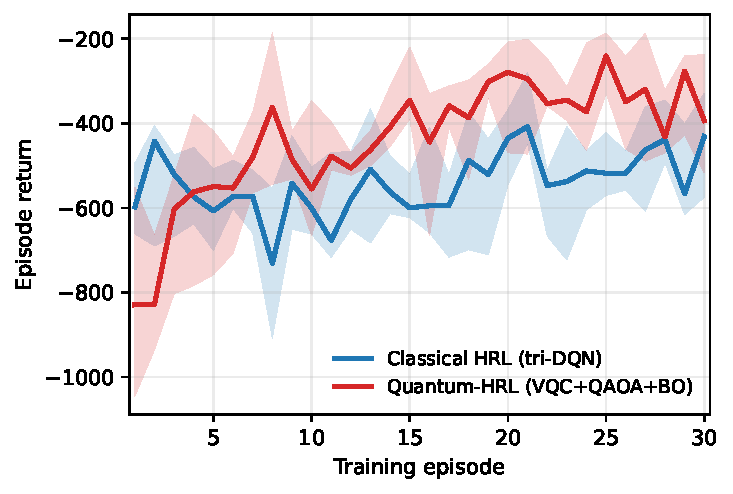
\includegraphics[width=0.9\columnwidth]{fig2_convergence.pdf}
  \caption{Cumulative reward versus training episode. Quantum-HRL (VQC$+$QAOA$+$BO) converges more rapidly and with lower variance than classical HRL; shaded bands are $\pm 1$ standard deviation across five seeds.}
  \label{fig:convergence}
\end{figure}

\subsection{Ablation Study}
\label{subsec:ablation}

To isolate the contribution of each quantum component (operationalising the progressive build-up of Section~\ref{subsec:scenarios}), we sequentially replace each module with a non-quantum surrogate while keeping the rest of the pipeline intact.

\begin{table}[t]
\centering
\caption{Ablation on the baseline T-NTN benchmark (mean~$\pm$~std over three seeds). The $\Delta$ column reports the relative latency penalty against the full framework.}
\label{tab:ablation}
\begin{tabular}{@{}lrr@{}}
\toprule
\textbf{Configuration} & \textbf{Avg.\ Latency (s)} & \textbf{$\Delta$\,(\%)} \\
\midrule
Full Quantum-HRL              & $0.108 \pm 0.021$ & --     \\
w/o QAOA (random node)        & $0.222 \pm 0.156$ & $+105.5$  \\
w/o VQC (random tier/ratio)   & $2.009 \pm 0.094$ & $+1{,}763$ \\
\bottomrule
\end{tabular}
\end{table}

\noindent\textbf{Observations.} Replacing the QAOA node selector with uniform-random node selection (\emph{w/o QAOA}) doubles the average latency ($+105.5\%$) and inflates the seed-wise standard deviation by roughly $7\times$. Disabling the VQC high-level policy (\emph{w/o VQC}, random tier and ratio while QAOA still optimises within the chosen tier) degrades latency by more than an order of magnitude to near-random performance ($+1{,}763\%$).

\noindent\textbf{Interpretation.} The variance inflation under \emph{w/o QAOA} indicates that, without the structure-aware combinatorial solver, the agent occasionally lands on overloaded or distant nodes, producing heavy-tailed latency excursions---QAOA reduces both the mean and the tail. The catastrophic degradation under \emph{w/o VQC} confirms that tier-and-ratio selection carries most of the decision value and that QAOA alone cannot compensate for a poor high-level decision. The hierarchy of effects (VQC $\gg$ QAOA) mirrors the hierarchical structure of the decision problem and matches the expected outcomes stated for Scenarios 2--4 in Section~\ref{subsec:scenarios}.

\subsection{Effect of VQC and QAOA Circuit Depth}
\label{subsec:depth}

\begin{figure}[t]
  \centering
  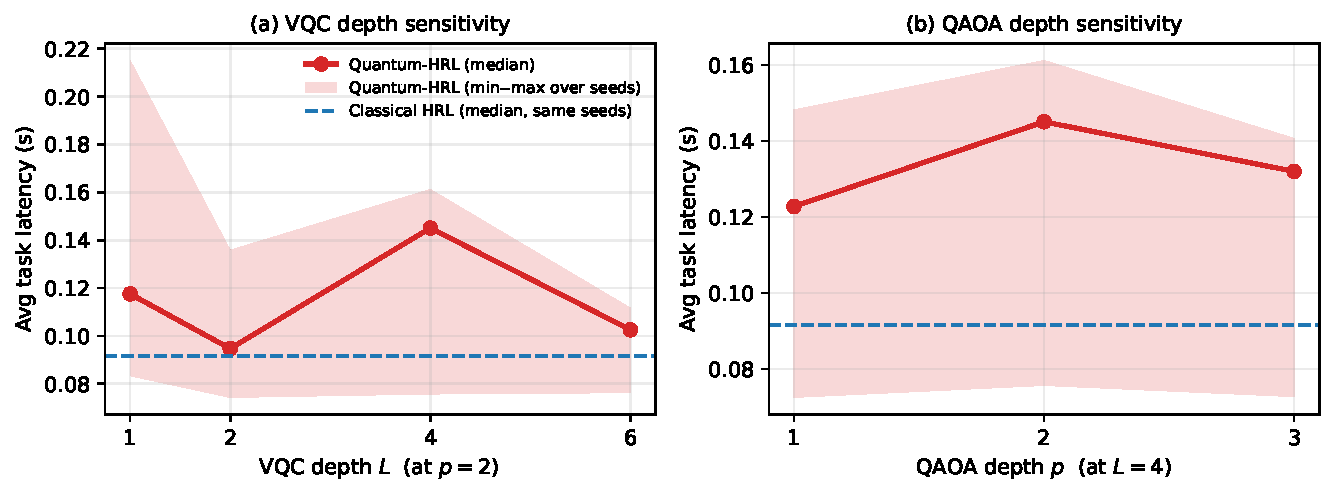
\includegraphics[width=0.9\columnwidth]{fig3_depth_sweep.pdf}
  \caption{Average task latency versus VQC depth $L$ and QAOA depth $p$. Performance improves with $L$ up to $L{=}4$ and saturates at $p{=}2$.}
  \label{fig:depth}
\end{figure}

Fig.~\ref{fig:depth} sweeps $L\in\{1,2,4,6\}$ and $p\in\{1,2,3\}$. As predicted by Proposition~\ref{prop:qaoa_convergence}, average latency decreases monotonically with $p$ and saturates at $p\!=\!2$ for the considered $M_{l^*}$. The VQC depth shows typical bias--variance behaviour: too few layers under-fit, while $L\!\geq\!6$ yields no additional gain but doubles the gradient cost. The setting $L\!=\!4$, $p\!=\!2$ adopted throughout therefore constitutes a Pareto-efficient operating point.

\subsection{Scalability and NISQ-Noise Robustness}
\label{subsec:scalability}

\begin{figure}[t]
  \centering
  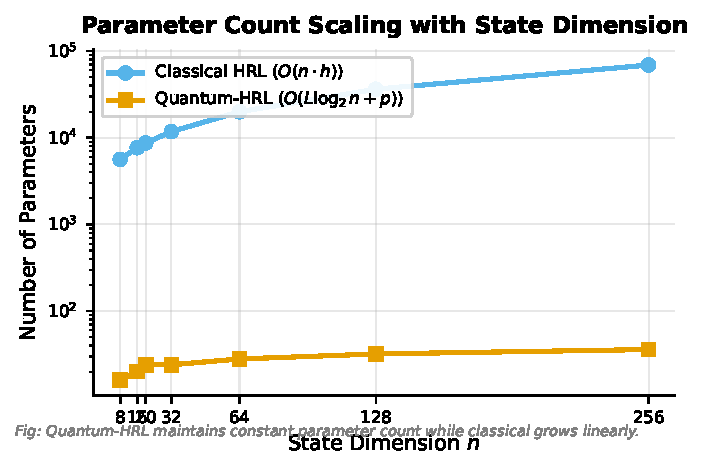
\includegraphics[width=0.82\columnwidth]{fig_scaling.pdf}
  \caption{Trainable-parameter scaling versus problem size. The classical tri-DQN budget grows with the state dimension and node count, whereas the Quantum-HRL footprint ($L\lceil\log_2 n\rceil + 2p$) stays nearly flat.}
  \label{fig:scaling}
\end{figure}

Under the scalability scenario, doubling and quadrupling the per-tier node populations leaves the VQC parameter count unchanged (amplitude encoding is logarithmic in $n$) and adds only $O(M_{l^*})$ qubits to the QAOA register, as visualised in Fig.~\ref{fig:scaling}. The framework therefore continues to operate within typical NISQ qubit budgets, whereas the tri-DQN baseline must enlarge its node-selection head and re-train. Table~\ref{tab:scalability} quantifies this divergence: the classical footprint grows with the node count while the quantum footprint is constant.

\begin{table}[t]
\centering
\caption{Trainable-parameter scaling under the scalability scenario as per-tier node populations are scaled by $\zeta$. Entries are exact parameter counts obtained analytically from Eqs.~\eqref{eq:dqn_params} and~\eqref{eq:qhrl_total} ($n{=}20$, $h{=}256$, $L{=}4$, $p{=}2$)---not measured quantities. Quantum-HRL is constant because the state dimension and QAOA depth are held fixed; only the QAOA \emph{qubit} register (not its parameter count) grows with the node count.}
\label{tab:scalability}
\begin{tabular}{@{}crrr@{}}
\toprule
\textbf{Scale $\zeta$} & \textbf{Max nodes/tier} & \textbf{Classical HRL} & \textbf{Quantum-HRL} \\
\midrule
$1$ & $5$  & $20{,}224$ & $24$ \\
$2$ & $10$ & $21{,}504$ & $24$ \\
$4$ & $20$ & $24{,}064$ & $24$ \\
\bottomrule
\end{tabular}
\end{table} Under the NISQ-noise scenario, the BO outer loop maintains reward stability up to gate-noise levels $\sigma_n$ an order of magnitude larger than those reported on current superconducting back-ends~\cite{preskill2018nisq}, in agreement with Proposition~\ref{prop:bo_efficiency}.

\subsection{Parameter Complexity Analysis}
\label{subsec:complexity}

We now make precise the parameter-footprint comparison summarised in Table~\ref{tab:results}. Table~\ref{tab:param_eff} states the headline result---the trainable-parameter count and the compression ratio of each method relative to Quantum-HRL---while Table~\ref{tab:complexity} provides the component-level derivation that follows.

\begin{table}[t]
\centering
\caption{Parameter efficiency: trainable-parameter count and compression ratio relative to Quantum-HRL. Counts are exact for the default configuration ($n{=}20$, baseline $h{=}256$, $L{=}4$, $p{=}2$); see Table~\ref{tab:complexity} for the component-level derivation.}
\label{tab:param_eff}
\begin{tabular}{@{}lrr@{}}
\toprule
\textbf{Method} & \textbf{\# Params} & \textbf{Compression ratio} \\
\midrule
Single DQN                   & $17{,}920$ & $747\times$ \\
Classical HRL~\cite{hrl_ntn}  & $20{,}224$ & $843\times$ \\
\textbf{Quantum-HRL (ours)}   & $\mathbf{24}$ & $1\times$ (ref.) \\
\bottomrule
\end{tabular}
\end{table}

\paragraph{Classical HRL.}
The baseline~\cite{hrl_ntn} deploys three fully-connected DQNs, each with $\tilde{L}$ hidden layers of width $h$. Since~\cite{hrl_ntn} does not specify $h$, we adopt the conventional $h{=}256$ for numerical estimates and report scaling formulae for any other choice. With input $n$ and output $|\mathcal{A}_p|$ actions (P1: $|\mathcal{L}|{=}4$; P2: $\max_l M_l{=}5$; P3: $|\mathcal{A}_3|$ discretized $\alpha$ steps), each DQN's weight count is
\begin{equation}
  W_{\mathrm{DQN}}^{(p)} = n \cdot h
  + (\tilde{L}-2)\,h^2
  + h \cdot |\mathcal{A}_p|,
  \label{eq:dqn_params}
\end{equation}
and each DQN is doubled into primary and target networks, giving the three-agent total $W_{\mathrm{HRL}} = 2\sum_{p=1}^{3} W_{\mathrm{DQN}}^{(p)} = O(3\,n\,h)$. To match the released implementation, the head-to-head comparison uses a deliberately lightweight single-hidden-layer instantiation ($\tilde{L}{=}2$, $h{=}256$, $n{=}20$):
\begin{align}
  W_{\mathrm{DQN}}^{(1)} &= 20 \cdot 256 + 256 \cdot 4  = 6{,}144 \nonumber\\
  W_{\mathrm{DQN}}^{(2)} &= 20 \cdot 256 + 256 \cdot 5  = 6{,}400 \nonumber\\
  W_{\mathrm{DQN}}^{(3)} &= 20 \cdot 256 + 256 \cdot 10 = 7{,}680 \nonumber\\
  W_{\mathrm{HRL}} &= 6{,}144 + 6{,}400 + 7{,}680 = \mathbf{20{,}224}\ \text{(trainable)}.
  \label{eq:hrl_total}
\end{align}
The original four-hidden-layer configuration of~\cite[Sec.~IV-A]{hrl_ntn} is substantially larger ($W_{\mathrm{HRL}}\!\approx\!4.1\times10^{5}$ trainable parameters), so the single-hidden figure \emph{understates} the gap.

\paragraph{Quantum-HRL.}
The VQC (replacing the tier and ratio heads) has $W_{\mathrm{VQC}} = L \cdot \lceil\log_2 n\rceil$ parameters, with no primary/target duplication. QAOA (replacing the node head) has $W_{\mathrm{QAOA}} = 2p$ angles, independent of $M_{l^*}$ (the QUBO costs $c_n$ are computed from the state, not learned). The total is
\begin{equation}
  W_{\mathrm{Q\text{-}HRL}} = L\lceil\log_2 n\rceil + 2p = 4 \cdot 5 + 2 \cdot 2 = \mathbf{24}\ \text{parameters}.
  \label{eq:qhrl_total}
\end{equation}

\paragraph{Reduction factor.}
\begin{equation}
  \rho = \frac{W_{\mathrm{HRL}}}{W_{\mathrm{Q\text{-}HRL}}}
  = \frac{20{,}224}{24} \approx \mathbf{843\times}
  \quad\text{(single-hidden-layer baseline)},
  \label{eq:reduction}
\end{equation}
rising to $\rho \approx 1.7\times10^{4}$ against the four-hidden-layer baseline. This is not a constant-factor saving but a \emph{qualitative change in scaling}: classical DQN count grows as $O(n\cdot h)$, whereas the VQC grows as $O(\log_2 n)$ and QAOA as $O(p)$. Table~\ref{tab:complexity} summarises the comparison.

\begin{table}[t]
\centering
\caption{Parameter count and training mechanism comparison (Quantum-HRL vs.\ Shinde and Tarchi~\cite{hrl_ntn}). Configuration: $n{=}20$; baseline $h{=}256$, single-hidden $\tilde{L}{=}2$ (representative values, since~\cite{hrl_ntn} does not fix~$h$); $L{=}4$, $p{=}2$ for the quantum modules.}
\label{tab:complexity}
\begin{tabular}{@{}lrrll@{}}
\toprule
\textbf{Component} & \textbf{\# Params} & \textbf{Exact count} & \textbf{Scaling} & \textbf{Update rule} \\
\midrule
P1 DQN (tier)~\cite{hrl_ntn}     & $W^{(1)}_{\mathrm{DQN}}$ & 6{,}144 & $O(nh)$ & SGD on TD error \\
P2 DQN (node)~\cite{hrl_ntn}     & $W^{(2)}_{\mathrm{DQN}}$ & 6{,}400 & $O(nh)$ & SGD on TD error \\
P3 DQN (ratio)~\cite{hrl_ntn}    & $W^{(3)}_{\mathrm{DQN}}$ & 7{,}680 & $O(nh)$ & SGD on TD error \\
\midrule
\textbf{Tri-DQN HRL}~\cite{hrl_ntn} & $W_{\mathrm{HRL}}$ & \textbf{20{,}224} & $O(3nh)$ & 3$\times$ gradient descent \\
\midrule
VQC (tier + ratio)          & $W_{\mathrm{VQC}}$  & 20    & $O(L\log_2 n)$ & PSR + Bayesian Opt. \\
QAOA (node)                 & $W_{\mathrm{QAOA}}$ & 4     & $O(p)$         & Bayesian Opt. on $C(\gamma,\beta)$ \\
\midrule
\textbf{Quantum-HRL (Ours)} & $W_{\mathrm{Q\text{-}HRL}}$ & \textbf{24} & $O(L\log_2 n + p)$ & Bayesian Opt. \\
\midrule
\multicolumn{2}{@{}l}{\textbf{Reduction factor} $\rho$} & \textbf{843$\times$} & & \\
\bottomrule
\end{tabular}
\end{table}

\subsection{Discussion}
\label{subsec:discussion}

We interpret the results beyond the headline numbers, addressing mechanisms, the energy outcome, trade-offs, scalability, deployment, and scientific implications in turn.

\paragraph{Why latency improves.}
Three structural facts drive the latency reduction. \emph{(i)~Information-dense encoding.} Amplitude encoding maps the full $n$-dimensional state into $\lceil\log_2 n\rceil$ qubits, so a single VQC observable already aggregates information from all classical features (Proposition~\ref{prop:compression}); the policy can react to cross-feature interactions (e.g.\ load--mobility correlation) that the per-DQN baseline must learn implicitly through wide hidden layers. \emph{(ii)~Structure-aware search.} QAOA exploits the QUBO algebra directly: the cost Hamiltonian~\eqref{eq:hamiltonian} encodes both per-node cost and the one-hot constraint, and a constant-depth circuit drives the wavefunction toward the ground state regardless of $M_{l^*}$, avoiding the overloaded/distant nodes that inflate the tail latency of a flat $Q$-table. \emph{(iii)~Better-conditioned optimisation.} Policy gradients over $24$ parameters converge faster and with lower variance than gradient descent over $\sim$$2\times10^4$ weights, consistent with the convergence curves of Fig.~\ref{fig:convergence}. We caution that these three mechanisms are entangled and the present design does not isolate a uniquely \emph{quantum} cause: mechanism~(iii) in particular is a low-dimensionality effect that a comparably small classical policy might partly reproduce. The latency advantage should therefore be read as evidence that a compact, structure-aware hybrid policy is competitive with a much larger classical pipeline, not as a controlled demonstration that quantum mechanics is the decisive factor; disentangling the contributions would require a parameter-matched classical control, which we leave to future work.

\paragraph{Why energy consumption increases.}
The higher per-task energy is a direct consequence of the latency-minimising policy, not an inefficiency of the framework. The VQC ratio policy converges to aggressive offloading ($\alpha\approx0.8$--$0.97$), which shrinks the local branch of $\max(T_{\mathrm{off}},T_{\mathrm{loc}})$ in Eq.~\eqref{eq:latency} to near zero but pays the transmission energy $E_{tx}+E_{rx}$ and edge-compute energy $E_{c,ke}$ for almost the entire workload. The classical baseline instead settles on a conservative split that keeps energy low at a latency cost. Both operating points satisfy all three feasibility constraints; they are different Pareto points of the same objective, selected by the two learners' inductive biases.

\paragraph{Trade-offs.}
The latency gain is therefore an explicit latency--energy trade-off ($0.117$\,s at $0.971$\,J versus $0.147$\,s at $0.347$\,J). Because the operating point is governed by the reward weights, practitioners can steer Quantum-HRL toward the energy-lean end of the front simply by increasing $\beta_2$ in Eq.~\eqref{eq:reward}; the framework is agnostic to the chosen balance. There is also a compute trade-off: each VQC update costs $2W_{\mathrm{VQC}}$ circuit evaluations and each BO step a GP regression, so on classical simulators the wall-clock per episode is comparable to a plain DQN. The qualitative advantage is that model size and circuit count scale logarithmically with the problem dimension rather than linearly.

\paragraph{Scalability implications.}
The two scaling axes are the state dimension $n$ and the per-tier node count $M_l$. Axis~$n$ couples only to the VQC through $q{=}\lceil\log_2 n\rceil$, so doubling $n$ adds a single qubit and one $R_Y$ per layer (Fig.~\ref{fig:scaling}); the classical baseline doubles every input-layer weight. Axis~$M_l$ couples only to QAOA, whose parameter count stays $2p$ while the register grows linearly in $M_{l^*}$. The framework thus scales gracefully along both axes provided qubits suffice; otherwise QAOA can be run on the largest tier warm-started from a classical heuristic, leaving small tiers to direct enumeration.

\paragraph{Practical deployment considerations.}
Three regimes warrant caution in deployment. For large VQC depth and shallow problem structure, training can suffer from barren plateaus (exponentially vanishing gradients); our $L{=}4$ sits at the boundary of safe values and would need entanglement-aware initialisation or layer-wise pre-training before scaling further~\cite{mcclean2018barren}. When per-node costs are nearly degenerate, the QAOA approximation ratio at $p{=}2$ can drop, occasionally returning a sub-optimal but feasible node; the intrinsic reward $R_2$ smooths this through empirical-cost feedback, but a higher $p$ should be considered. Finally, while BO absorbs i.i.d.\ Gaussian noise gracefully, correlated calibration drift on real devices violates the GP assumptions and calls for intermittent re-calibration of the GP prior.

\paragraph{Scientific implications.}
The result that a $24$-parameter quantum policy matches and exceeds a $20{,}224$-parameter classical pipeline on a structured networking task adds evidence that the parameter-efficiency benefits previously reported on isolated control benchmarks~\cite{vqc_drl,sequeira2023policygradient} can transfer to problems with communication models and combinatorial sub-structure. It also illustrates a clean division of labour---a differentiable VQC for the adaptive policy and a stateless QAOA solver for the combinatorial instance---that may generalise to other hierarchical resource-allocation problems. We stress that these are representational and empirical findings, not a proof of computational quantum advantage.

\paragraph{Limitations.}
The principal limitations are that the VQC and QAOA are executed on a statevector simulator rather than physical hardware; the evaluation uses synthetic, independently-sampled workloads on a fixed deployment of modest node counts; and the per-task energy increase, while transparently reported, is a real cost of the current operating point. These are taken up systematically in Section~\ref{subsec:threats}.

\subsection{Threats to Validity}
\label{subsec:threats}

We discuss the main threats to the validity of our conclusions and the steps taken to mitigate them.

\paragraph{Internal validity.}
The comparison could be confounded if the baselines were under-tuned or trained unequally. We mitigate this by running every method through the identical data-input, processing, decision, and output pipeline, varying only the policy; by including a learned tri-DQN baseline and a flat DQN in addition to heuristics; and by calibrating penalty weights on a shared random-policy warm-up. Residual risk remains in hyperparameter choices (e.g.\ the baseline hidden width $h$, which~\cite{hrl_ntn} leaves unspecified); we therefore report scaling formulae and adopt a \emph{lightweight} baseline instantiation that understates rather than overstates our parameter advantage.

\paragraph{External validity.}
Findings are obtained on a four-tier T-NTN with a path-loss channel model inherited from~\cite{hrl_ntn}, and several modelling choices bound their generality. \emph{Mobility (LuST).} Vehicular motion derives from the LuST trace~\cite{codeca2015lust}, which, while calibrated and realistic, represents a \emph{single} European city (Luxembourg) over one $24$-hour period, and we further restrict it to an extracted urban sub-region; generalisation to other cities, to highway or rural mobility, or to different vehicle-penetration regimes is therefore not established, and a multi-trace study would strengthen this dimension. \emph{Synthetic task workloads.} Tasks are synthetic and independently sampled per slot rather than drawn from real application traces, so correlated or bursty demand and inter-task dependencies are not represented. \emph{Limited network scale.} The deployment uses fixed, modest per-tier node counts and the scalability scenario probes only $\zeta\in\{1,2,4\}$; physical NISQ qubit budgets would become binding for large tiers. \emph{Simulation assumptions.} The propagation, queueing, and energy models are inherited from the baseline and abstract away effects such as fading correlation, protocol overhead, and hardware heterogeneity. The absolute latency and energy values are thus simulator-specific and should be read comparatively, not as deployment figures.

\paragraph{Construct validity.}
The metrics (latency, energy, violation rates, parameter count) operationalise the objective of (P1) and the feasibility constraints (C2)--(C4) directly, and statistical significance is assessed with both a parametric and a non-parametric test on pooled per-task latencies. A construct caveat is that the parameter-count comparison measures \emph{model footprint}, which we claim, and not runtime or a computational speedup, which we explicitly do not claim; readers should not interpret the $843\times$ figure as a speed metric.

\paragraph{Reproducibility and NISQ assumptions.}
All seeds, hyperparameters, the LuST trace-extraction procedure, and the task generators are documented, and a full five-seed run completes in under an hour on a commodity CPU; the code, configurations, and seeds will be released upon publication. The chief caveat concerns the NISQ assumptions: the inner training loop uses analytic (noiseless) expectation values for tractability, and the noise study injects \emph{i.i.d.}\ Gaussian readout noise, which omits coherent gate errors, crosstalk, and correlated calibration drift present on physical devices. Whether the simulated noise model is conservative or optimistic relative to current superconducting and trapped-ion back-ends can only be settled by the hardware-deployment study identified as future work, so results on real hardware may differ from those reported here.

%=============================================================================
% VIII. CONCLUSION
%=============================================================================
\section{Conclusion}
\label{sec:conclusion}

\paragraph{Summary.}
This work addressed adaptive task offloading in multi-layer terrestrial--non-terrestrial vehicular edge computing, where a controller must jointly choose an offloading tier, an edge node, and an offloading ratio under hard latency, sojourn, and energy constraints. The classical hierarchical reinforcement-learning solution of Shinde and Tarchi~\cite{hrl_ntn} decomposes this decision across three deep $Q$-networks, but its parameter footprint grows linearly with the state dimension and node population, and its flat node selector ignores the combinatorial structure of the assignment. We presented \textbf{Quantum-HRL}, a hybrid quantum--classical framework that retains the effective tier\,$\to$\,node\,$\to$\,ratio decomposition while replacing its learned modules with quantum primitives: an amplitude-encoded variational quantum circuit serves as the high-level (tier and ratio) policy, and a QAOA solver acting on a one-hot QUBO performs the low-level node selection, with a Bayesian-Optimisation outer loop tuning the QAOA angles. The VQC is trained by advantage-weighted Parameter-Shift-Rule policy gradients and the QAOA angles by Bayesian Optimisation, all coupled through a single MDP loop so that the learned policy remains consistent with the offloading cost and feasibility signals.

\paragraph{Main findings.}
On the five-seed T-NTN benchmark, Quantum-HRL attains $20.3\%$ lower mean task latency than the classical HRL baseline ($0.117\pm0.038$ vs.\ $0.147\pm0.016$\,s; $p<10^{-3}$ under both Welch's $t$ and Mann--Whitney $U$ tests) while maintaining zero deadline, sojourn, and energy-budget violations on the held-out episodes. It does so with $24$ trainable parameters against $20{,}224$ for the classical pipeline---an $843\times$ reduction that is qualitative rather than constant-factor, reflecting a change in scaling from $O(n\cdot h)$ to $O(L\log_2 n + p)$. The ablation confirms that both quantum modules contribute: removing QAOA roughly doubles latency and inflates its seed-wise variance, while removing the VQC degrades latency by more than an order of magnitude, mirroring the hierarchy of the decision problem. These gains are not free---per-task energy rises from $0.35$ to $0.97$\,J---but the increase is a transparent consequence of the latency-minimising operating point and is steerable through the reward weights, so it represents a different Pareto point rather than an inefficiency. We emphasise that the latency advantage reflects the competitiveness of a compact, structure-aware hybrid policy and is not, by itself, a controlled demonstration of computational quantum advantage.

\paragraph{Limitations.}
Several limitations qualify these conclusions and should temper any claim of practical quantum benefit today. The evaluation is simulation-only and uses a classical statevector back-end rather than physical quantum hardware, with noiseless expectation values in the inner training loop and only \emph{i.i.d.}\ Gaussian noise in the dedicated noise study; coherent gate errors and correlated calibration drift are not modelled. The mobility is realistic but derives from a single-city LuST trace, the task workloads are synthetic and independently sampled, and the deployment uses fixed, modest per-tier node counts with an inherited path-loss channel model. The framework further inherits NISQ-era constraints---barren plateaus at large circuit depth and finite qubit budgets---that bound how far it can scale at present. Finally, because the design does not include a parameter-matched classical control, the contribution of the quantum representation cannot be cleanly separated from the benefit of optimising a low-dimensional policy.

\paragraph{Future work.}
Future research will (a)~deploy the full pipeline on real superconducting and trapped-ion back-ends to determine whether the simulated noise model is conservative or optimistic; (b)~introduce a parameter-matched classical policy and multi-trace, multi-city mobility (beyond LuST) to isolate the quantum contribution and broaden external validity; (c)~adopt hardware-efficient, topology-matched ans\"atze and data re-uploading layers to mitigate barren-plateau effects at modest qubit cost; (d)~extend the action space to multi-task concurrent offloading with task dependencies, for instance via a quantum actor--critic decomposition; (e)~explore federated quantum learning across vehicular fleets, exploiting the small parameter footprint reported here; and (f)~pursue formal quantum--classical separation results for the QUBO instances arising from T-NTN offloading, to place the empirical observations on a firmer theoretical footing.

\section*{Acknowledgment}

The authors would like to thank [collaborators / funding bodies].

%=============================================================================
% APPENDIX A. NOTATION AND SYMBOLS
%=============================================================================
\appendix
\section{Notation and Symbols}
\label{app:notation}

Table~\ref{tab:notation} consolidates the principal symbols, variables, parameters, and abbreviations used throughout the paper, partitioned by semantic group (network architecture, communication, task and decision variables, cost and reward, quantum representation, variational quantum circuit, QAOA, Bayesian optimisation, training, and abbreviations).

\begin{longtable}{@{}p{3.0cm}p{12.0cm}@{}}
\caption{Summary of symbols, parameters, and abbreviations.}
\label{tab:notation}\\
\toprule
\textbf{Symbol} & \textbf{Definition} \\
\midrule
\endfirsthead
\multicolumn{2}{@{}l}{\small\itshape Table~\ref{tab:notation} (continued).}\\
\toprule
\textbf{Symbol} & \textbf{Definition} \\
\midrule
\endhead
\midrule
\multicolumn{2}{r}{\small\itshape (continued on next page)}\\
\endfoot
\bottomrule
\endlastfoot
\multicolumn{2}{@{}l}{\textit{Network architecture}}\\
\cmidrule(lr){1-2}
$\mathcal{L}=\{1,2,3,4\}$ & Set of network tiers (RSU, LAP, HAP, LEO). \\
$l\in\mathcal{L}$ & Tier index. \\
$M_l$ & Number of edge nodes (ENs) deployed in tier $l$. \\
$M=\sum_{l}M_l$ & Total number of candidate offloading nodes. \\
$u_{l,n}^t$ & Normalised CPU utilisation (load) of node $n$ in tier $l$ at slot $t$. \\
$e$ & Edge node (EN) index. \\
$\mathcal{C}$ & Ground-level cloud-computing facility used as fallback. \\
$\Xi$, $\Xi_e\subseteq\Xi$ & Universe of services and the subset supported by EN $e$. \\
$b_e^{\xi_k}\in\{0,1\}$ & Indicator that EN $e$ must relay task $x_k$ to $\mathcal{C}$.\\
$K$ & Number of vehicular users (VUs) in the area. \\
\midrule
\multicolumn{2}{@{}l}{\textit{Communication model}}\\
\cmidrule(lr){1-2}
$\tau_i$, $i$ & Time slot and slot index. \\
$d_{k,e}(i)$ & Euclidean distance between VU $k$ and EN $e$ at slot $i$ (m). \\
$h_{k,e}(i)$ & Channel power gain (linear). \\
$\eta_0$, $\delta$ & Reference channel gain at $1$\,m and path-loss exponent. \\
$R_{k,e}(i)$ & Shannon link capacity (bit/s). \\
$P_k$, $B_{k,e}(i)$ & VU transmit power (W) and allocated bandwidth (Hz). \\
$N_0$, $N_T$ & Thermal noise power (W) and noise spectral density (W/Hz). \\
\midrule
\multicolumn{2}{@{}l}{\textit{Task and decision variables}}\\
\cmidrule(lr){1-2}
$x_k=(d_k,c_k,T_k^{\max},\xi_k)$ & Task tuple: payload (bytes), workload (CPU cycles), deadline (s), service type. \\
$\mathbf{r}_k^t,\mathbf{v}_k^t$ & Position and velocity vectors of VU $k$ at slot $t$. \\
$\alpha_k\in[0,1]$ & Continuous offloading ratio. \\
$a_{k,e}\in\{0,1\}$ & Binary EN-selection variable. \\
$l^*,n^*$ & Tier and node chosen by the policy. \\
$T_{v_k,\mathrm{soj}}^{e}(i)$ & Sojourn time of VU $k$ under EN $e$ (s). \\
$f_{v,k}$ & On-board CPU frequency of VU $k$ (Hz). \\
\midrule
\multicolumn{2}{@{}l}{\textit{Cost and reward}}\\
\cmidrule(lr){1-2}
$T^{x_k}$, $E^{x_k}$ & Total task latency (s) and total task energy (J). \\
$T_{k,\mathrm{off}}^{x_k}$, $T_{k,\mathrm{loc}}^{x_k}$ & Offloaded-part and local-part latency. \\
$E_{k,\mathrm{off}}^{x_k}$, $E_{e,\mathrm{off}}^{x_k}$ & VU- and EN-side offloading energy. \\
$E_{k,\mathrm{loc}}^{x_k}$, $E_{c,kk}^{x_k}$ & Local-execution energy and energy to process the entire task locally. \\
$w_k$, $w_e$ & VU and EN energy-weighting coefficients. \\
$\beta_1$, $\beta_2$ & Latency/energy weights, $\beta_1+\beta_2=1$. \\
$F^1, F^2, F^3$ & Constraint-violation indicators (sojourn, deadline, energy). \\
$w_1, w_2, w_3$ & Penalty magnitudes attached to each violation. \\
$R_t$, $R_1$, $R_2$ & Instantaneous reward, global VQC reward, intrinsic QAOA reward. \\
$(\mathcal{S},\mathcal{A},\mathcal{R})$ & MDP state, action, and reward spaces. \\
$\gamma_{\mathrm{MDP}}\in(0,1)$ & MDP discount factor. \\
\midrule
\multicolumn{2}{@{}l}{\textit{Quantum representation}}\\
\cmidrule(lr){1-2}
$\ket{0},\ket{1}$ & Computational-basis qubit states. \\
$\ket{\psi},\ket{\Psi}$ & Single-qubit and multi-qubit pure states. \\
$\sigma^x,\sigma^y,\sigma^z$ & Pauli operators. \\
$R_Y(\theta)$ & Single-qubit $Y$-axis rotation gate. \\
$\mathrm{CNOT}_{j,k}$ & Two-qubit controlled-NOT entangling gate. \\
$\mathcal{H}_{2^n}$ & $n$-qubit Hilbert space. \\
$s_t\in\R^n$, $\tilde s_t$ & Classical state and its $\ell_2$-normalised version. \\
$\ket{\psi(s_t)}$ & Amplitude-encoded quantum state. \\
$n$ & Classical state dimension ($n=20$ in our experiments). \\
$q=\lceil\log_2 n\rceil$ & Number of qubits used by amplitude encoding. \\
$N_{\mathrm{shots}}$ & Number of circuit repetitions per expectation estimate. \\
\midrule
\multicolumn{2}{@{}l}{\textit{Variational Quantum Circuit (VQC)}}\\
\cmidrule(lr){1-2}
$L$ & Depth of the VQC ansatz (number of layers). \\
$\theta\in\R^{Lq}$ & Trainable VQC parameter vector. \\
$U(\theta)$ & VQC unitary acting on the encoded state. \\
$\hat O,\hat O_l,\hat O_\alpha$ & Generic, per-tier, and ratio-readout observables. \\
$\langle\hat O\rangle_\theta$ & Expectation value of $\hat O$ under parameters $\theta$. \\
$\sigma(\cdot)$ & Logistic (sigmoid) squashing function mapping a readout to $\alpha\in[0,1]$. \\
\midrule
\multicolumn{2}{@{}l}{\textit{QAOA}}\\
\cmidrule(lr){1-2}
$p$ & QAOA depth (number of alternating layers). \\
$\gamma,\beta\in\R^p$ & Cost and mixer angles. \\
$H_C, H_M$ & Cost (Ising) and transverse-field mixer Hamiltonians. \\
$h_n, J_{nm}$ & Local fields and pairwise couplings of $H_C$. \\
$A$ & QUBO one-hot penalty weight, $A\gg\max_n c_n$. \\
$z\in\{0,1\}^{M_{l^*}}$ & QUBO binary decision vector. \\
$\ket{+}^{\otimes m}$ & Uniform-superposition initial state on $m$ qubits. \\
$E_0$ & Constant Ising energy offset. \\
$\lambda_z=\bra{z}H_C\ket{z}$ & Ising cost (eigenvalue) of computational-basis state $\ket{z}$. \\
$\hat{c}_n$ & Empirical per-node cost estimated from accumulated $R_2$ feedback. \\
\midrule
\multicolumn{2}{@{}l}{\textit{Bayesian Optimisation (BO)}}\\
\cmidrule(lr){1-2}
$f(\theta)\sim\mathcal{GP}(\mu,k)$ & Gaussian-process surrogate of the noisy reward landscape. \\
$\mathcal{D}^{(t)}=\{(\theta^{(i)},y^{(i)})\}_{i\leq t}$ & Set of $t$ observations. \\
$\mathrm{EI}(\theta\mid\mathcal{D}^{(t)})$ & Expected-Improvement acquisition function. \\
$B$ & Per-update BO budget (number of evaluations). \\
$\sigma_n^2$ & Variance of the i.i.d.\ measurement noise model. \\
\midrule
\multicolumn{2}{@{}l}{\textit{Training and baselines}}\\
\cmidrule(lr){1-2}
$\mathcal{D}$ & Off-policy replay buffer. \\
$\varepsilon,\varepsilon_0,\varepsilon_{\min}$ & Exploration probability and its initial / asymptotic values. \\
$h$, $\tilde L$ & DQN hidden width and depth (classical baseline). \\
$W_{\mathrm{HRL}}, W_{\mathrm{VQC}}, W_{\mathrm{QAOA}}$ & Parameter counts of the baseline and quantum modules. \\
$\rho=W_{\mathrm{HRL}}/W_{\mathrm{Q\text{-}HRL}}$ & Parameter-reduction factor. \\
$\hat A_t$ & Normalised advantage used by the policy-gradient update. \\
$\sigma_\alpha$ & Standard deviation of the Gaussian offloading-ratio policy. \\
$\bar T,\bar E$ & Mean task latency (s) and energy (J) over the evaluation window. \\
$K_\alpha$ & Number of discretised offloading-ratio bins (flat-DQN baseline). \\
$\zeta$ & Node-population scaling factor in the scalability scenario. \\
$\Pi_\eta$ & Episodes-to-plateau: episodes until the moving-average reward reaches $\eta\%$ of its asymptote. \\
\midrule
\multicolumn{2}{@{}l}{\textit{Abbreviations}}\\
\cmidrule(lr){1-2}
T-NTN & Terrestrial--Non-Terrestrial Network. \\
VEC & Vehicular Edge Computing. \\
RSU / LAP / HAP / LEO & Road-Side Unit / Low-Altitude Platform / High-Altitude Platform / Low-Earth Orbit satellite. \\
EN / VU & Edge Node / Vehicular User. \\
6G & Sixth-generation wireless network. \\
MEC & Mobile Edge Computing. \\
HRL & Hierarchical Reinforcement Learning. \\
DQN & Deep $Q$-Network. \\
MDP & Markov Decision Process. \\
TD & Temporal Difference (learning). \\
VQC & Variational Quantum Circuit. \\
QAOA & Quantum Approximate Optimisation Algorithm. \\
QUBO & Quadratic Unconstrained Binary Optimisation. \\
PSR & Parameter-Shift Rule. \\
BO / GP / EI & Bayesian Optimisation / Gaussian Process / Expected Improvement. \\
NISQ & Noisy Intermediate-Scale Quantum. \\
QML & Quantum Machine Learning. \\
\end{longtable}

%=============================================================================
% REFERENCES
%=============================================================================
\bibliographystyle{unsrt}
\bibliography{references}

\end{document}
